% Options for packages loaded elsewhere
\PassOptionsToPackage{unicode}{hyperref}
\PassOptionsToPackage{hyphens}{url}
%
\documentclass[
  doc, donotrepeattitle,floatsintext]{apa7}
\usepackage{amsmath,amssymb}
\usepackage{lmodern}
\usepackage{iftex}
\ifPDFTeX
  \usepackage[T1]{fontenc}
  \usepackage[utf8]{inputenc}
  \usepackage{textcomp} % provide euro and other symbols
\else % if luatex or xetex
  \usepackage{unicode-math}
  \defaultfontfeatures{Scale=MatchLowercase}
  \defaultfontfeatures[\rmfamily]{Ligatures=TeX,Scale=1}
\fi
% Use upquote if available, for straight quotes in verbatim environments
\IfFileExists{upquote.sty}{\usepackage{upquote}}{}
\IfFileExists{microtype.sty}{% use microtype if available
  \usepackage[]{microtype}
  \UseMicrotypeSet[protrusion]{basicmath} % disable protrusion for tt fonts
}{}
\makeatletter
\@ifundefined{KOMAClassName}{% if non-KOMA class
  \IfFileExists{parskip.sty}{%
    \usepackage{parskip}
  }{% else
    \setlength{\parindent}{0pt}
    \setlength{\parskip}{6pt plus 2pt minus 1pt}}
}{% if KOMA class
  \KOMAoptions{parskip=half}}
\makeatother
\usepackage{xcolor}
\usepackage{graphicx}
\makeatletter
\def\maxwidth{\ifdim\Gin@nat@width>\linewidth\linewidth\else\Gin@nat@width\fi}
\def\maxheight{\ifdim\Gin@nat@height>\textheight\textheight\else\Gin@nat@height\fi}
\makeatother
% Scale images if necessary, so that they will not overflow the page
% margins by default, and it is still possible to overwrite the defaults
% using explicit options in \includegraphics[width, height, ...]{}
\setkeys{Gin}{width=\maxwidth,height=\maxheight,keepaspectratio}
% Set default figure placement to htbp
\makeatletter
\def\fps@figure{htbp}
\makeatother
\setlength{\emergencystretch}{3em} % prevent overfull lines
\providecommand{\tightlist}{%
  \setlength{\itemsep}{0pt}\setlength{\parskip}{0pt}}
\setcounter{secnumdepth}{-\maxdimen} % remove section numbering
% Make \paragraph and \subparagraph free-standing
\ifx\paragraph\undefined\else
  \let\oldparagraph\paragraph
  \renewcommand{\paragraph}[1]{\oldparagraph{#1}\mbox{}}
\fi
\ifx\subparagraph\undefined\else
  \let\oldsubparagraph\subparagraph
  \renewcommand{\subparagraph}[1]{\oldsubparagraph{#1}\mbox{}}
\fi
\newlength{\cslhangindent}
\setlength{\cslhangindent}{1.5em}
\newlength{\csllabelwidth}
\setlength{\csllabelwidth}{3em}
\newlength{\cslentryspacingunit} % times entry-spacing
\setlength{\cslentryspacingunit}{\parskip}
\newenvironment{CSLReferences}[2] % #1 hanging-ident, #2 entry spacing
 {% don't indent paragraphs
  \setlength{\parindent}{0pt}
  % turn on hanging indent if param 1 is 1
  \ifodd #1
  \let\oldpar\par
  \def\par{\hangindent=\cslhangindent\oldpar}
  \fi
  % set entry spacing
  \setlength{\parskip}{#2\cslentryspacingunit}
 }%
 {}
\usepackage{calc}
\newcommand{\CSLBlock}[1]{#1\hfill\break}
\newcommand{\CSLLeftMargin}[1]{\parbox[t]{\csllabelwidth}{#1}}
\newcommand{\CSLRightInline}[1]{\parbox[t]{\linewidth - \csllabelwidth}{#1}\break}
\newcommand{\CSLIndent}[1]{\hspace{\cslhangindent}#1}
\ifLuaTeX
\usepackage[bidi=basic]{babel}
\else
\usepackage[bidi=default]{babel}
\fi
\babelprovide[main,import]{english}
% get rid of language-specific shorthands (see #6817):
\let\LanguageShortHands\languageshorthands
\def\languageshorthands#1{}
% Manuscript styling
\usepackage{upgreek}
\captionsetup{font=singlespacing,justification=justified}

% Table formatting
\usepackage{longtable}
\usepackage{lscape}
% \usepackage[counterclockwise]{rotating}   % Landscape page setup for large tables
\usepackage{multirow}		% Table styling
\usepackage{tabularx}		% Control Column width
\usepackage[flushleft]{threeparttable}	% Allows for three part tables with a specified notes section
\usepackage{threeparttablex}            % Lets threeparttable work with longtable

% Create new environments so endfloat can handle them
% \newenvironment{ltable}
%   {\begin{landscape}\centering\begin{threeparttable}}
%   {\end{threeparttable}\end{landscape}}
\newenvironment{lltable}{\begin{landscape}\centering\begin{ThreePartTable}}{\end{ThreePartTable}\end{landscape}}

% Enables adjusting longtable caption width to table width
% Solution found at http://golatex.de/longtable-mit-caption-so-breit-wie-die-tabelle-t15767.html
\makeatletter
\newcommand\LastLTentrywidth{1em}
\newlength\longtablewidth
\setlength{\longtablewidth}{1in}
\newcommand{\getlongtablewidth}{\begingroup \ifcsname LT@\roman{LT@tables}\endcsname \global\longtablewidth=0pt \renewcommand{\LT@entry}[2]{\global\advance\longtablewidth by ##2\relax\gdef\LastLTentrywidth{##2}}\@nameuse{LT@\roman{LT@tables}} \fi \endgroup}

% \setlength{\parindent}{0.5in}
% \setlength{\parskip}{0pt plus 0pt minus 0pt}

% Overwrite redefinition of paragraph and subparagraph by the default LaTeX template
% See https://github.com/crsh/papaja/issues/292
\makeatletter
\renewcommand{\paragraph}{\@startsection{paragraph}{4}{\parindent}%
  {0\baselineskip \@plus 0.2ex \@minus 0.2ex}%
  {-1em}%
  {\normalfont\normalsize\bfseries\itshape\typesectitle}}

\renewcommand{\subparagraph}[1]{\@startsection{subparagraph}{5}{1em}%
  {0\baselineskip \@plus 0.2ex \@minus 0.2ex}%
  {-\z@\relax}%
  {\normalfont\normalsize\itshape\hspace{\parindent}{#1}\textit{\addperi}}{\relax}}
\makeatother

% \usepackage{etoolbox}
\makeatletter
\patchcmd{\HyOrg@maketitle}
  {\section{\normalfont\normalsize\abstractname}}
  {\section*{\normalfont\normalsize\abstractname}}
  {}{\typeout{Failed to patch abstract.}}
\patchcmd{\HyOrg@maketitle}
  {\section{\protect\normalfont{\@title}}}
  {\section*{\protect\normalfont{\@title}}}
  {}{\typeout{Failed to patch title.}}
\makeatother

\usepackage{xpatch}
\makeatletter
\xapptocmd\appendix
  {\xapptocmd\section
    {\addcontentsline{toc}{section}{\appendixname\ifoneappendix\else~\theappendix\fi\\: #1}}
    {}{\InnerPatchFailed}%
  }
{}{\PatchFailed}
\keywords{Motor learning, OPTIMAL theory, Publication bias, Z-curve}
\usepackage{csquotes}
\usepackage{pdflscape}
\usepackage{longtable}
\usepackage{graphicx}
\usepackage{graphbox}
\usepackage{tabularray}
\UseTblrLibrary{booktabs}
\raggedbottom
\renewcommand\author[1]{}
\renewcommand\affiliation[1]{}
\authorsnames[1, 2, 3, 3, 1]{Brad McKay, Mariane F.B. Bacelar, Juliana O. Parma, Matthew W. Miller\textsuperscript{$\dagger$}, Michael J. Carter\textsuperscript{$\dagger$}\vspace{2ex}}
\authorsaffiliations{{Department of Kinesiology, McMaster University}, {Department of Kinesiology, Boise State University}, {School of Kinesiology, Auburn University}}
\ifLuaTeX
  \usepackage{selnolig}  % disable illegal ligatures
\fi
\IfFileExists{bookmark.sty}{\usepackage{bookmark}}{\usepackage{hyperref}}
\IfFileExists{xurl.sty}{\usepackage{xurl}}{} % add URL line breaks if available
\urlstyle{same} % disable monospaced font for URLs
\hypersetup{
  pdftitle={The combination of reporting bias and underpowered study designs have substantially exaggerated the motor learning benefits of self-controlled practice and enhanced expectancies: A meta-analysis},
  pdflang={en-EN},
  pdfkeywords={Motor learning, OPTIMAL theory, Publication bias, Z-curve},
  hidelinks,
  pdfcreator={LaTeX via pandoc}}

\title{The combination of reporting bias and underpowered study designs have substantially exaggerated the motor learning benefits of self-controlled practice and enhanced expectancies: A meta-analysis}
\author{\phantom{0}}
\date{}


\shorttitle{Motivation pillar of OPTIMAL theory}

\authornote{

\vspace{-0.5cm}

\noindent \textsuperscript{$\dagger$}Co-Senior Authors \newline
\newline
\noindent \addORCIDlink{Brad McKay}{0000-0002-7408-2323} \newline
\noindent \addORCIDlink{Mariane F.B. Bacelar}{0000-0002-0388-1769} \newline
\noindent \addORCIDlink{Juliana O. Parma}{0000-0002-3118-9921} \newline
\noindent \addORCIDlink{Matthew W. Miller}{0000-0002-7896-7217} \newline
\noindent \addORCIDlink{Michael J. Carter}{0000-0002-0675-4271} \newline       
\newline
\noindent Data and code: \url{https://osf.io/vfza7/} \newline
\newline
\noindent \textbf{Corresponding authors:} Brad McKay (\href{mailto:bradmckay8@gmail.com}{\nolinkurl{bradmckay8@gmail.com}}; \href{mailto:mckayb9@mcmaster.ca}{\nolinkurl{mckayb9@mcmaster.ca}}) and Michael J. Carter (\href{mailto:michaelcarter@mcmaster.ca}{\nolinkurl{michaelcarter@mcmaster.ca}}; \href{mailto:motorlab@mcmaster.ca}{\nolinkurl{motorlab@mcmaster.ca}})

}

\affiliation{\phantom{0}}

\abstract{%
Enhanced expectancies and autonomy-support through self-controlled practice conditions form the motivation pillar of OPTIMAL theory (Wulf \& Lewthwaite, 2016). The influence of these practice variables on motor learning was recently evaluated in two separate meta-analyses. Both meta-analyses found that the published literature suggested a moderate and significant benefit on motor learning; however, evidence for reporting bias was found in both literatures. Although multiple bias-corrected estimates were reported in the self-controlled meta-analysis, there was no principled way to prefer one over the other. In the enhanced expectancies meta-analysis, the trim-and-fill-technique failed to correct the estimated effects. Here, we addressed these limitations by reanalyzing the data from both meta-analyses using robust Bayesian meta-analysis methods. Our reanalysis revealed that reporting bias substantially exaggerated the benefits of these practice variables in the original meta-analyses. The true effects are instead small, uncertain, and potentially null. We also found the estimated average statistical power among all studies from the original meta-analyses was 6\% (95\% confidence interval {[}5\%, 13\%{]}). These results provide compelling and converging evidence that strongly suggests the available literature is insufficient to support the motivation pillar of OPTIMAL theory. Our results highlight the need for adequately powered experimental designs if motor learning scientists want to make evidence-based recommendations.
}



\begin{document}
\maketitle

For nearly 20 years, motor learning and performance research has been accumulating that some (e.g., Wulf et al., 2010; Wulf \& Lewthwaite, 2016, 2021) have argued is not well-explained by classic information-processing-based theories (Guadagnoli \& Lee, 2004; Salmoni et al., 1984; Schmidt, 1975). Examples range from putative motor learning benefits from receiving bogus social comparison feedback (e.g., Ávila et al., 2012) to ostensive learning and performance enhancement as a consequence of making incidental choices during practice (e.g., Lewthwaite et al., 2015). In the Optimizing Performance Through Intrinsic Motivation and Attention for Learning (OPTIMAL) theory, Wulf and Lewthwaite (2016) argued that the failure of information-processing theories to account for findings like these created the need for a new theory of motor learning. The OPTIMAL theory provided an account of these, and numerous other lines of research, proposing that autonomy support and enhanced expectancies increase motivation, which explains the learning and performance benefits observed with self-controlled practice (see Sanli et al., 2013 for a review), positive feedback (e.g., Chiviacowsky \& Wulf, 2007), social comparative feedback (e.g., Ávila et al., 2012), perceived task difficulty (e.g., C. Lee et al., 2011), conceptions of ability (e.g., Cimpian et al., 2007), self-modeling (e.g., Ste-Marie et al., 2011), and extrinsic rewards (e.g., Abe et al., 2011). While motivation had been deemphasized in previous motor learning theories, within OPTIMAL theory numerous lines of 21st century research may be best explained by motivational rather than informational mechanisms.

Unfortunately, it has become recognized throughout social science that reporting bias in the literature can seriously distort the evidence (Collaboration, 2015; Fanelli, 2010; Hagger et al., 2016; Munafò et al., 2017). The results explained by the motivational factors in OPTIMAL theory may therefore be exaggerated or even non-existent (Gelman \& Carlin, 2014). Research on the motor learning literature specifically has found evidence of the pernicious combination of low statistical power, high multiplicity (i.e., many statistical tests), and selective reporting (Lohse et al., 2016). The evidence underpinning the autonomy support predictions in OPTIMAL theory has been questioned in a recent meta-analysis, suggesting that low power combined with reporting bias may be responsible for the apparent benefits of self-controlled practice (McKay et al., in-press). In that study, it was observed that published experiments found an average self-controlled practice benefit of \emph{g} = .54. However, several models of reporting bias provided a better fit to the data than the naive random effects model. Each of the models suggested the true average effect was small or potentially zero. Self-controlled practice was the primary literature addressed by the autonomy support factor in OPTIMAL theory; yet, these findings call into question whether there was even a robust phenomenon to explain.

Bacelar and colleagues (2022) investigated the literature addressed by the second motivation factor in OPTIMAL theory---enhanced expectancies. In their meta-analysis, Bacelar and colleagues found that the average benefit of studies that manipulated expectancies via interventions described in OPTIMAL theory was \emph{g} = .54. However, there was evidence of reporting bias that could not be accounted for with moderators in the study. The authors applied the trim-and-fill method in an effort to adjust for reporting bias, but it made no corrections and no other corrections were applied. It is noteworthy that self-controlled practice studies and the studies included in the Bacelar et al.~meta-analysis have much in common: both literatures are comprised of variables predicted by OPTIMAL theory to increase motivation and in turn motor performance and learning; both include studies examined in a meta-analysis by Lohse and colleagues (2016) that found evidence of low power, multiplicity, and bias; and both showed signs of reporting bias in their funnel plots. If both literatures have been affected similarly by reporting bias, then the current estimate of \emph{g} = .54 for variables thought to enhance expectancies may be a substantial overestimate.

Addressing reporting bias presents substantial challenges to meta-analysts. Since reporting bias limits the information we have access to, it is impossible to know for certain how much bias is present or how large the impact is (Carter et al., 2019; McShane et al., 2016). The best we can do is think carefully about the mechanisms that potentially underlie reporting bias and attempt to model them accurately. In contrast, a naive random effects analysis assumes there is no reporting bias. Complicating matters, reporting bias can take several different forms with unique impacts on the final sample (Maier et al., in-press; Stefan \& Schönbrodt, 2022; Thornton \& Lee, 2000). To account for this, multiple models of reporting bias need to be attempted without knowing which is most likely \emph{a priori}. Thus, bias-correction analyses are inherently sensitivity analyses (Mathur \& VanderWeele, 2020; Sutton et al., 2000; Vevea \& Woods, 2005). Until recently, if the results of multiple sensitivity analyses differed widely, there was no mechanism to reconcile the estimates. We now have Robust Bayesian Meta-Analysis (RoBMA) methods that apply Bayesian model averaging to allow meta-analysts to fit several plausible models (see Table \ref{tab:table1} for descriptions) and give greater weight to the models that best account for the data (Bartoš et al., 2022; Maier et al., in-press). The RoBMA method provides single estimates of the average effect and heterogeneity, along with Bayes factors to quantify the evidence in support of a true effect, the presence of heterogeneity, and the presence of reporting bias. Results from simulation studies and analyses of real data with known reporting bias mechanisms suggest that RoBMA is substantially more accurate and less biased than naive random effects models and also performs better than other competing reporting bias models (Bartoš et al., 2022).

\clearpage

\renewcommand{\arraystretch}{1.7}
\DefTblrTemplate{caption-tag}{default}{Table\hspace{0.25em}\thetable}
\DefTblrTemplate{caption-sep}{default}{.\enskip}
\DefTblrTemplate{caption-text}{default}{\InsertTblrText{caption}}
\DefTblrTemplate{contfoot-text}{default}{(\emph{Continued})}
\DefTblrTemplate{middlehead,lasthead}{default}{\textbf{Table 1.} Continued}
\SetTblrStyle{caption-tag,caption-sep}{\bfseries}
\small
\begin{longtblr}[
  caption = {The selection and regression models used in our robust Bayesian meta-analysis approach.},
  label = {tab:table1},
]{colspec = {p{4.5cm}p{5cm}p{4.5cm}}}
\toprule
  \textbf{Type of selection} &
  \textbf{Visualization} &
  \textbf{Example scenario} \\ 
\midrule
  \textbf{\underline{Selection models}} &
  &
  \textbf{\underline{Direction not important}} \\
Significant results are more likely to be reported in either direction (two-tailed)  &
  \raisebox{-0.9\height}{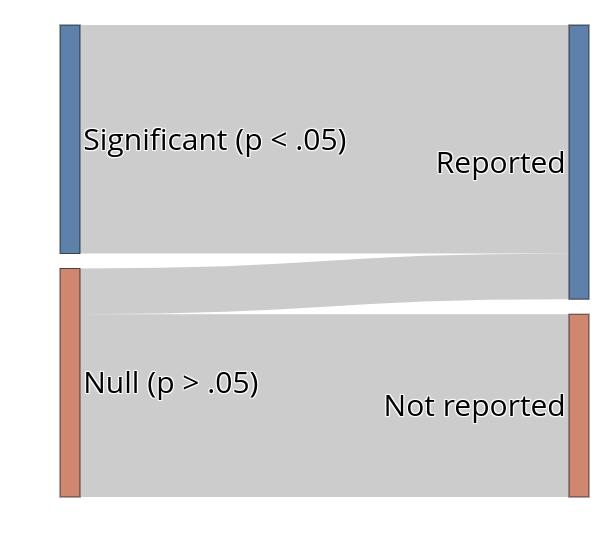
\includegraphics[width=4.75cm]{../../figs/model1.png}} &
  Researcher conducts test and observes a null result. They decide the experiment did not work and move on. Significant results get reported. \\
Significant results are most likely to be reported, but ``non-significant trends'' are more likely to be reported than other null results in either direction (two-tailed). &
  \raisebox{-0.9\height}{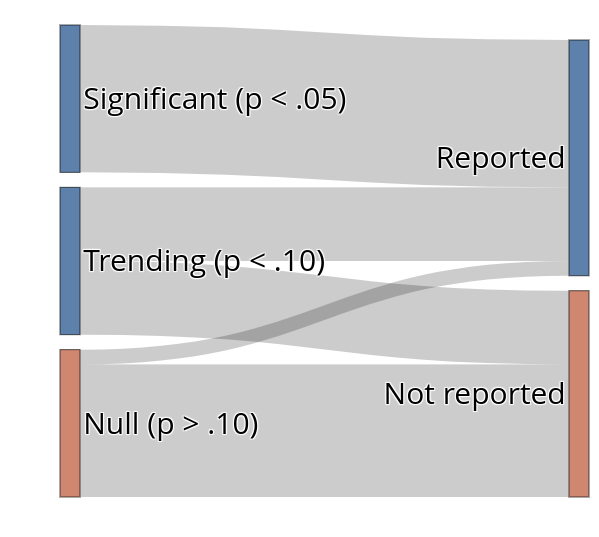
\includegraphics[width=4.75cm]{../../figs/model2.png}} &
  Authors report significant results and ``non-significant trends''. The latter may be interpreted as fair evidence the manipulation worked. Some reviewers take issue with trends, so only some make it through and get reported. Null results unlikely to be written up. \vspace{1em} \\
  &
  &
  \textbf{\underline{Direction important}} \\
Significant results and non-significant trends are more likely to be reported in the predicted direction. &
  \raisebox{-0.9\height}{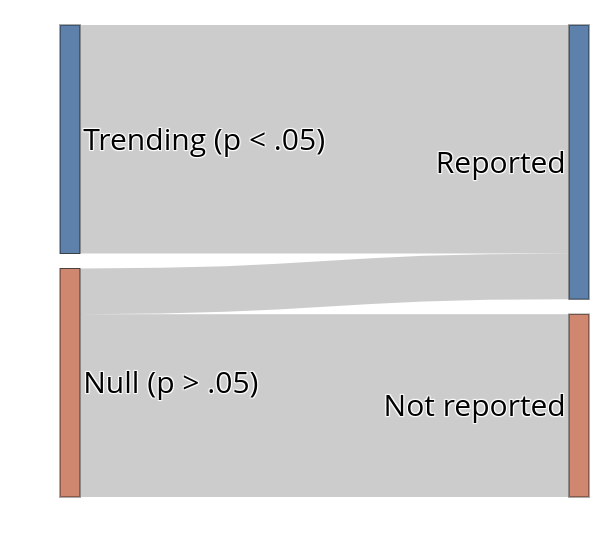
\includegraphics[width=4.75cm]{../../figs/model3.png}} &
  Researcher is confident in the hypothesis being tested in an experiment and doubts the validity of null or opposing findings. Reports results they are confident in. \\
Significant results in the predicted direction are more likely to be reported than trends, which are more likely to be reported than other null results and significant results in the opposite (i.e., ``wrong'') direction. &
  \raisebox{-0.9\height}{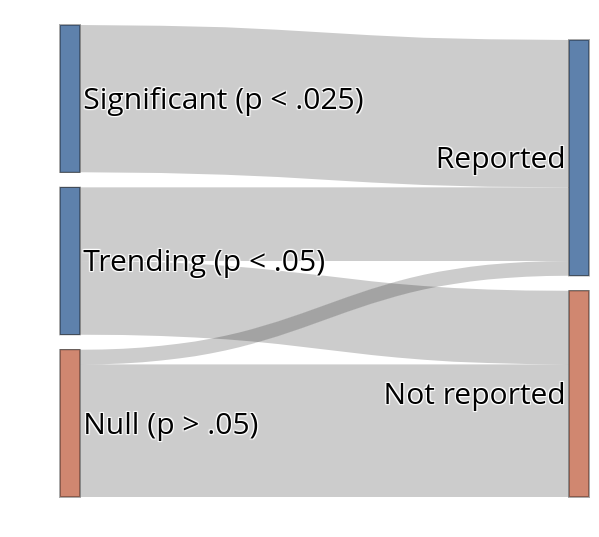
\includegraphics[width=4.75cm]{../../figs/model4.png}} &
  A preference for reporting findings with a compelling narrative results in preferring significant results and occasionally trends. Null or conflicting results less likely to add to the narrative. \\
Significant results and trends in the predicted (i.e., ``correct'') direction are more likely to be reported than null findings in the predicted (i.e., ``correct'') direction, which are more likely to be reported than results in the opposite (i.e., ``wrong'') direction. &
  \raisebox{-0.9\height}{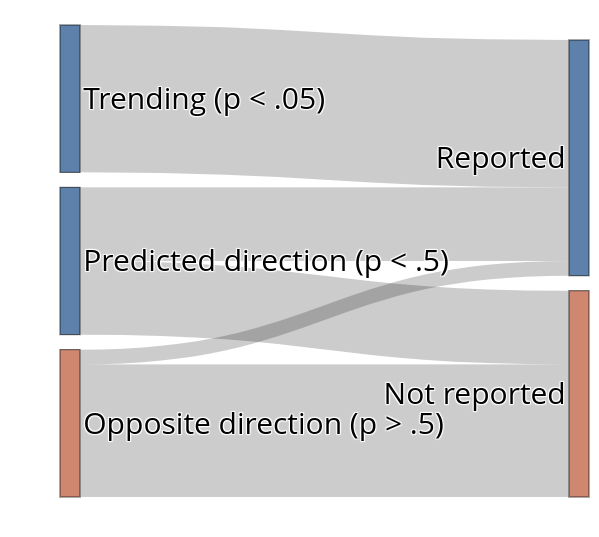
\includegraphics[width=4.75cm]{../../figs/model5.png}} &
  A student observes results in the opposite direction of what was expected. Supervisor thinks something may have went wrong so results not published. Other students publish results consistent with predictions. \\
Full selection model. Significant results most likely, then trends, then null results in the predicted (i.e., ``correct'') direction. The least likely to be reported are results in the opposite (i.e., ``wrong'') direction. &
  \raisebox{-0.9\height}{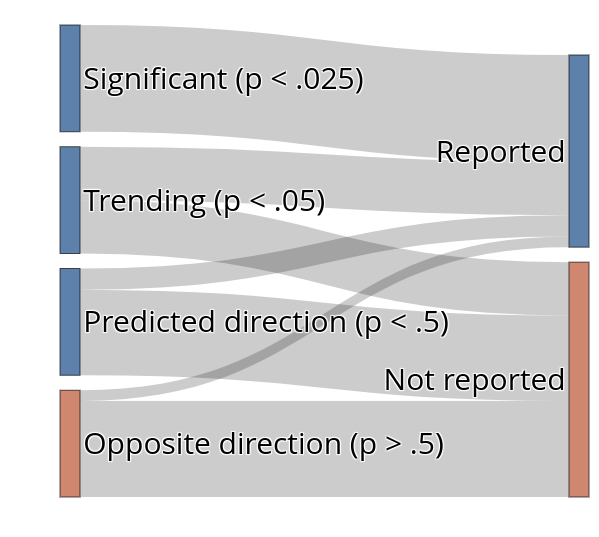
\includegraphics[width=4.75cm]{../../figs/model6.png}} &
  An editor prefers to publish interesting results. Prediction successes are interesting. Some trends are interesting if they are believable. Results in the opposite direction are interesting, but only if replicated. \\
  \textbf{\underline{Regression models}} &
  &
  \\
Conditioning on smaller \emph{p}-values in the predicted direction creates a relationship between effect sizes and standard errors. Called ``small study effects'' because all else being equal smaller studies need larger effects to achieve significant results. &
  \raisebox{-0.9\height}{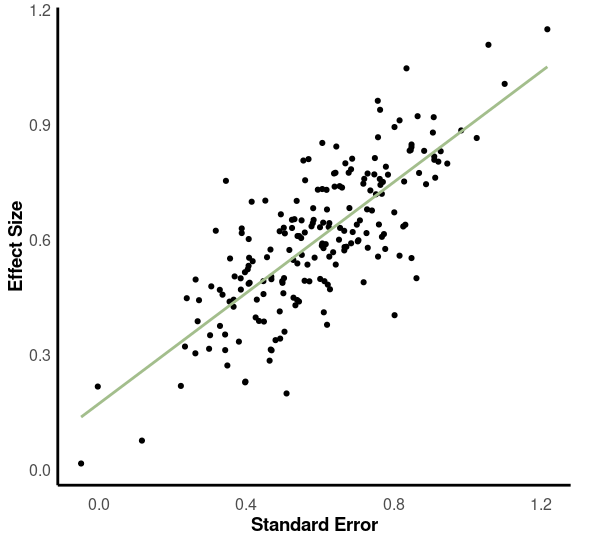
\includegraphics[width=4.75cm]{../../figs/model7.png}} &
  This models the dependency caused by selective reporting, not the underlying mechanism itself. Dependency can be caused by a third variable, such as intensity of the interventions used in smaller compared to larger studies. \\
Quadratic relationship between effect and standard errors. Large studies likely to be reported independent of results, while smaller studies need increasingly large effects in the predicted (i.e., ``correct'') direction to avoid censorship. &
  \raisebox{-0.9\height}{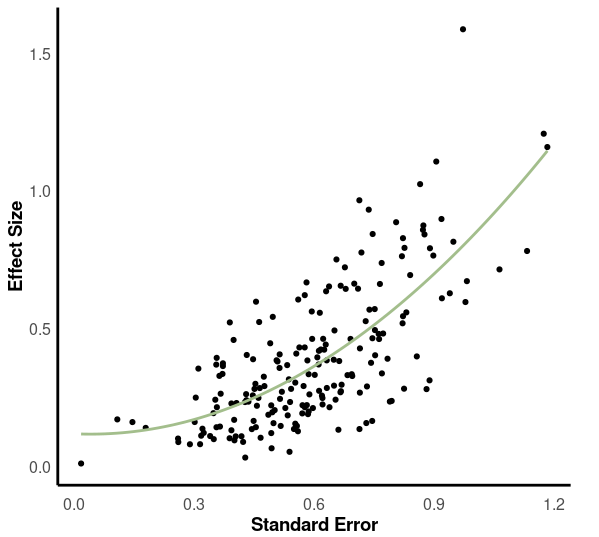
\includegraphics[width=4.75cm]{../../figs/model8.png}} &
  Researchers invest in conducting a large study and are motivated to publish regardless of the results. They persevere if null results are rejected. Small studies are abandoned unless the results are impressive. \\
\bottomrule
\end{longtblr}

\clearpage

\normalsize

A challenge for most reporting bias models is large heterogeneity in true effects. While RoBMA appears to perform well with moderate levels of heterogeneity, its performance has not been evaluated when heterogeneity is high and the performance of each of its constituent reporting bias models suffers with high heterogeneity (Carter et al., 2019). The \emph{z}-curve model was designed specifically to perform well regardless of heterogeneity (Bartoš \& Schimmack, in-press). While \emph{z}-curve does not provide adjusted effect size estimates (and such estimates may be meaningless with high heterogeneity), it instead estimates the average underlying power of included experiments. A significant difference between the estimated power of studies and the observed proportion of significant results can indicate the presence of reporting bias in a literature.

Here, we leveraged state-of-the-art robust Bayesian meta-analysis and \emph{z}-curve methods to re-analyze the meta-analyses by McKay and colleagues (in-press) and Bacelar and colleagues (2022). Considering the potential importance of OPTIMAL theory for the field of motor learning and performance (see T. D. Lee \& Carnahan, 2021 for a discussion), it is imperative that the evidence buttressing its motivation predictions be evaluated as rigorously as possible. Critically, our re-analysis addresses limitations in both previous meta-analyses. First, the analysis of enhanced expectancies fit only one bias correction model---the trim-and-fill method (Duval \& Tweedie, 1998)---and that model has been shown to result in exaggerated effect size estimates and severely inflated Type 1 error rates in the presence of publication bias and small or null effects (Bartoš et al., 2022; Carter et al., 2019). Second, although the results from multiple reporting bias models coalesced around small effect sizes (ranged from \emph{g} = -.11 to \emph{g} = .26) in the analysis of self-controlled practice, there are no principled reasons for preferring one estimate over another. We now consider a wider range of plausible models of reporting bias than that used in the previous meta-analyses. We also leverage Bayesian model averaging to upweight the best performing models, which has the advantage of evaluating single model-averaged posterior distributions for each parameter of interest. Lastly, we fit \emph{z}-curve models to the data in both meta-analyses. With this technique, the average power can be estimated and compared to the rate of significant results, providing crucial insight into the quality of the evidence-base supporting motivation predictions in OPTIMAL theory.

\hypertarget{materials-and-methods}{%
\section{Materials and methods}\label{materials-and-methods}}

Data and code used in this study can be accessed using either of the following links: \url{https://osf.io/vfza7/} or \url{https://github.com/cartermaclab/proj_sc-ee-optimal-theory}.

\hypertarget{description-of-datasets}{%
\subsection{Description of datasets}\label{description-of-datasets}}

The original meta-analyses followed similar inclusion criteria and data extraction policies (see Figure \ref{fig:fig1}). All data were extracted by two independent researchers with conflicts settled by including a third researcher. The literature search ended in August of 2019 in the self-controlled practice meta-analysis, and 10 months later in June 2020 in the enhanced expectancies meta-analysis.

\begin{figure}

{\centering 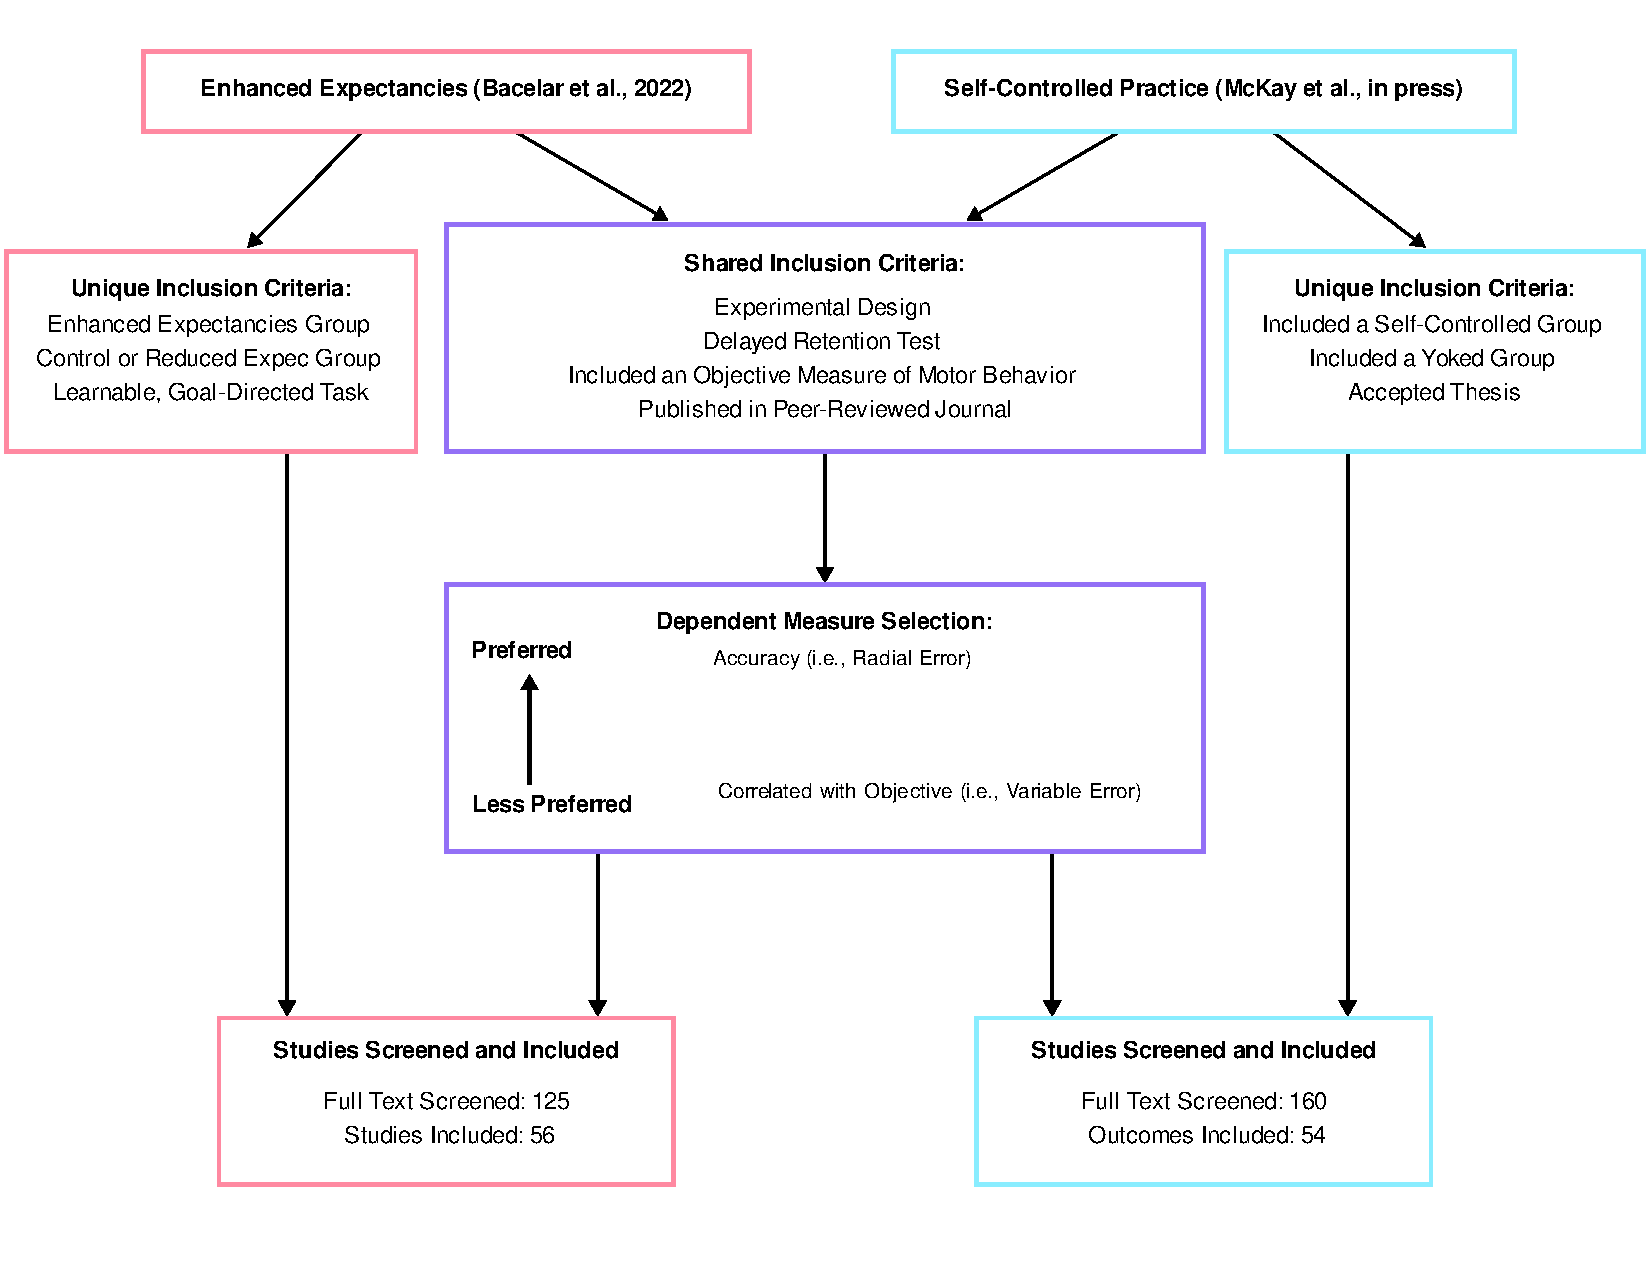
\includegraphics{../../figs/fig1} 

}

\caption{\normalfont \small \textbf{Inclusion criteria, dependent variable selection, studies screended and outcomes included in each meta-analysis.}}\label{fig:fig1}
\end{figure}



\hypertarget{robust-bayesian-meta-analysis}{%
\subsection{Robust Bayesian meta-analysis}\label{robust-bayesian-meta-analysis}}

The self-controlled practice and enhanced expectancy meta-data were reanalyzed using robust Bayesian meta-analysis with publication selection model-averaging (RoBMA-PSMA) (Maier et al., in-press). The RoBMA-PSMA method evaluates the evidence for reporting bias and adjusts effect size estimates and 95\% credible intervals to account for the estimated bias. Since the true data generating process underlying the data is unknown, the RoBMA-PSMA method fits several plausible models to the data. The models vary with respect to whether a) an effect is present or absent, b) there is one true effect (fixed effect) or a true average effect (random effects), c) reporting bias is present or absent, and d) if present, how results are selected for publishing.

Two classes of models are included to account for selective publishing of results. The first class of models are known as selection models. In a selection model, a weight-function based on \emph{p}-values is fit to the data and the probability that a result survives censorship to be included in the model is estimated for each \emph{p}-value interval. For example, a one-tailed \emph{p}-value cut point of .025 might be specified, corresponding to a two-sided \emph{p}-value of .05 in the positive direction. The probability that non-significant results survive censorship is estimated relative to the probability that positive significant results are published, which is set at 1. Selection models can be used to model a variety of potential forms of selective publishing. For example, selection may be concerned with significance but not the direction of the effect; in which case a two-sided \emph{p}-value of .05 can be fit to the model. Selection may also be based on both statistical significance in the positive direction and the direction of the point estimate; in which case one-sided \emph{p}-values of .025 and .5 can be fit to the model. The RoBMA-PSMA method fits six different selection models corresponding to various plausible forms of selection based on discrete \emph{p}-values.

The second class of models fit in the RoBMA-PSMA method model the relationship between observed effect sizes and their standard errors. A positive relationship between effect sizes and their standard errors has been termed ``small study effects'' (Sterne et al., 2000). The RoBMA-PSMA includes the precision-effect test (PET) and the precision-effect test with standard errors (PEESE) for small study effects. The PET model fits the relationship between observed effect sizes and their standard errors, while the PEESE model instead includes the square of the standard errors (i.e., their variances). The difference between the PET and PEESE models is that the PET model fits a linear relationship between the effect observed in a study and the precision with which that effect was estimated. The PEESE model fits a quadratic relationship. Thus, the PET and PEESE models differ with respect to the assumed underlying selection process. The PET model assumes that effect sizes increase in step with decreases in precision, consistent with selection based on statistical significance. The PEESE model assumes that studies with high precision are likely to be published regardless of statistical significance, whereas increasingly imprecise studies require increasingly larger effect size estimates to survive censorship.

RoBMA includes 36 separate models: a) six weight-function selection models in each level of a 2 (Effect: present, absent) x 2 (Heterogeneity: present, absent) matrix (24 models in total), b) PET and PEESE regression models in each level of the 2 x 2 Effect x Heterogeneity matrix (8 models in total), and c) models assuming no reporting bias at each level of the Effect x Heterogeneity matrix (4 models in total). The prior probabilities for the reporting-bias adjusted and unadjusted models are both set to .5; thus, summing to 1.0. The prior for the reporting-bias adjusted models is spread evenly between the selection and PET-PEESE regression model classes, so the priors for the two model classes sum to .5. Estimates from all 36 models are combined using Bayesian model-averaging, which weights each model estimate based on its posterior probability. Models that better account for the data are given greater weight in the RoBMA-PSMA model and models that provide a poor fit are down-weighted. The adjusted effect size estimate is produced by averaging across all models. This preserves the uncertainty about the true data generating process while weighting the component models based on their relative performance.

In addition to providing an overall effect estimate, the RoBMA-PSMA model can also be used to calculate Bayes factors (BF) quantifying the strength of support for the presence (or absence) of an intervention effect, heterogeneity, or reporting bias. To illustrate, consider the question of whether there is or is not an intervention effect. Since we used a neutral prior that considered each possibility equally likely, we can take the ratio of the posterior probabilities of model ensembles that included an effect to those that did not. We always report the BFs so they can be interpreted as how many times more likely the data were assuming the best supported hypothesis compared to the other hypothesis. For example, a BF01 = 2.0 for the absence of an intervention effect suggests that the models assuming all variation is random fit the data twice as well as models predicting an effect is present\footnote{BF\textsubscript{10} is the inverse of BF\textsubscript{01}, so while BF\textsubscript{01} indicates evidence in support of the null hypothesis, BF\textsubscript{10} indicates evidence in support of the alternative hypothesis.}. Bayes factors should be interpreted as a continuous measure of the relative support for one hypothesis versus another, not as the probability a hypothesis is true.

RoBMA-PSMA outperforms other meta-analytic approaches, including each constituent model included in RoBMA-PSMA, in simulations covering a range of plausible scenarios (Maier et al., in-press). Further, an analysis of real data from an approximately known data generating process (multi-lab registered replication report) suggested that RoBMA-PSMA outperforms other available techniques (Bartoš \& Schimmack, in-press). These strong performance indices combined with the ability to simultaneously model various plausible manifestations of reporting bias made RoBMA-PSMA an attractive choice for re-analyzing the enhanced expectancies and self-controlled practice meta-analyses.

\hypertarget{z-curve}{%
\subsection{\texorpdfstring{\emph{Z}-curve}{Z-curve}}\label{z-curve}}

The self-controlled practice meta-data\footnote{\emph{Z}-curve results for self-controlled practice were reported previously in McKay et al. (in-press). We reproduce them here for comparison to enhanced expectancies and motivational factors combined analyses.}, enhanced expectancy meta-data, and the combination of both the enhanced expectancy and self-controlled practice meta-data were analyzed with a \emph{z}-curve. A \emph{z}-curve analysis estimates the statistical power of all studies ever conducted within a given literature, even if those studies were not reported, on the basis of the significant results that are present (Bartoš et al., 2022). That power estimate is equivalent to the expected discovery rate, that is, the expected rate of significant results for a given literature. The expected discovery rate estimated by a \emph{z}-curve and its corresponding 95\% confidence interval can be compared to the observed discovery rate in the literature (the actual rate of significant results). A discrepancy between the 95\% confidence interval of the expected discovery rate estimate and the observed discovery rate provides evidence of reporting bias.

\emph{Z}-curve analyzes two-tailed \emph{p}-values or absolute \emph{z}-scores, which do not preserve the direction of the effect and therefore follow a folded normal distribution. Because the selection process that determines whether non-significant results survive censorship is unknown, \emph{z}-curve includes only significant results. Therefore, the expected distribution of \emph{z}-scores in a \emph{z}-curve analysis is a folded normal distribution truncated at \emph{z} = 1.96, corresponding to the conventional threshold for statistical significance. \emph{Z}-curve is intended to be applied in both standard meta-analytic situations as well as broader investigations of entire fields, journals, or researcher publication histories. Therefore, the expected distribution of \emph{z}-values in \emph{z}-curve is heterogeneous, forming a mixture of truncated folded normal distributions with means equal to the population mean for each study and a standard deviation of 1. Critically, the mixture of truncated folded normal distributions for a given set of significant studies is a function of the average power of the population of studies from which they were sampled. By approximating this distribution \emph{z}-curve can estimate the average power of all studies conducted within a given literature, the so-called expected discovery rate. \emph{Z}-curve estimates the mixture model by using the expectation maximization algorithm (Dempster et al., 1977; G. Lee \& Scott, 2012) to fit a finite mixture model of seven truncated folded normal distributions with population means of 0, 1, 2, 3, 4, 5, and 6.

Similar to RoBMA-PSMA (Maier et al., in-press), \emph{z}-curve has also performed well in simulation studies and when applied to multi-lab registered replication data (Bartoš \& Schimmack, in-press). \emph{Z}-curve is a tool that can provide insight into the possible power shortcomings of a particular literature. Further, as \emph{z}-curve was designed to accommodate highly heterogeneous inputs, it is ideal for exploring power and reporting bias among studies that used a variety of methods to manipulate the two motivational factors in Wulf and Lewthwaite's (2016) OPTIMAL theory of motor learning.

\hypertarget{data-analysis}{%
\subsection{Data analysis}\label{data-analysis}}

We fit two RoBMA-PSMA models to the enhanced expectancies meta-data using the effect sizes and variances calculated by Bacelar and colleagues (2022). The first model included all studies, while the second excluded two influential cases, consistent with the primary results reported in the original meta-analysis. The self-controlled practice effect sizes and standard errors reported by McKay and colleagues (in-press) were analyzed using the same strategy.

\emph{Z}-curve models were fit to the enhanced expectancy and self-controlled practice meta-data separately, as well as combined. The same strategy was followed regarding influential cases. For all analyses, the model excluding influential cases is reported in detail and models with all studies included are discussed only when there are meaningful differences.

Statistical analyses were conducted using R (Version 4.2.1; R Core Team, 2021) and the R-packages \emph{geomtextpath} (Version 0.1.0; Cameron \& van den Brand, 2022), \emph{gt} (Version 0.6.0; Iannone et al., 2022), \emph{invgamma} (Version 1.1; Kahle \& Stamey, 2017), \emph{metafor} (Version 3.4.0; Viechtbauer, 2010), \emph{papaja} (Version 0.1.0.9999; Aust \& Barth, 2020), \emph{patchwork} (Version 1.1.0.9000; Pedersen, 2022), \emph{plotly} (Version 4.10.0; Sievert, 2020), \emph{pwr} (Version 1.3.0; Champely, 2020), \emph{renv} (Version 0.15.5; Ushey, 2022), \emph{robma} (Bartoš \& Maier, 2020), \emph{tidyverse} (Version 1.3.1; Wickham et al., 2019), \emph{tinylabels} (Version 0.2.3; Barth, 2022), \emph{truncdist} (Version 1.0.2; Novomestky \& Nadarajah, 2016), and \emph{zcurve} (Version 2.1.2; Bartoš \& Schimmack, 2020) were used in this project.

\hypertarget{results}{%
\section{Results}\label{results}}

\hypertarget{robust-bayesian-meta-analysis-1}{%
\subsection{Robust Bayesian meta-analysis}\label{robust-bayesian-meta-analysis-1}}

\hypertarget{self-controlled-practice}{%
\subsubsection{Self-controlled practice}\label{self-controlled-practice}}

The model-averaged posterior distribution of the average effect from the RoBMA-PSMA model is displayed in Figure \ref{fig:fig1}B. The results suggest moderate evidence against the presence of an effect, BF\textsubscript{01} = 3.16, very weak evidence against the presence of heterogeneity, BF\textsubscript{rf} = 1.7, and overwhelming evidence for the presence of reporting bias, BF\textsubscript{pb} = 18,399. The overall model ensemble estimated the effect of self-controlled practice as \emph{d} = .034 (95\% credible interval {[}.0, .248{]}). Heterogeneity was estimated as \(\tau\) = .05 (95\% credible interval {[}.0, .261{]}). A model fit with two influential cases included found overwhelming evidence for the presence of heterogeneity, BF\textsubscript{rf} = 1,924,516 and estimated \(\tau\) = .559 (95\% credible interval {[}.36, .78{]}). There were no other meaningful differences between models.

\hypertarget{enhanced-expectancies}{%
\subsubsection{Enhanced expectancies}\label{enhanced-expectancies}}

The model-averaged posterior distribution of the average effect from the RoBMA-PSMA model is displayed in Figure \ref{fig:fig1}C. The results revealed weak evidence for the presence of an effect BF\textsubscript{10} = 1.9, weak evidence for the presence of reporting bias, BF\textsubscript{pb} = 2.3, and very strong evidence for the presence of heterogeneity, BF\textsubscript{rf} = 47.6. The model ensemble estimated an average effect of \emph{d} = .26 (95\% credible interval {[}-.07, .63{]}). Heterogeneity was estimated as \(\tau\) = .35 (95\% credible interval {[}.07, .54{]}). A model fit with two influential cases included found weak evidence for the absence of an effect BF\textsubscript{01} = 2.5, strong evidence for the presence of reporting bias, BF\textsubscript{pb} = 21, and overwhelming evidence for the presence of heterogeneity, BF\textsubscript{rf} = 45,300. The model ensemble estimated an average effect of \emph{d} = .00 (95\% credible interval {[}-.62, .59{]}), \(\tau\) = .49 (95\% credible interval {[}.32, .68{]}).

The RoBMA-PSMA models with and without influential cases differed primarily with respect to the fit of the PEESE models. When two large effect sizes with large standard errors were included in the analysis, the PEESE model provided a very strong fit to the data (BF\textsubscript{10} = 39.9) when assuming no true effect but the presence of heterogeneity. When the two influential cases were excluded, the best fitting model was the PET under the same assumptions (BF\textsubscript{10} = 9.4).

\clearpage

\begin{figure}

{\centering 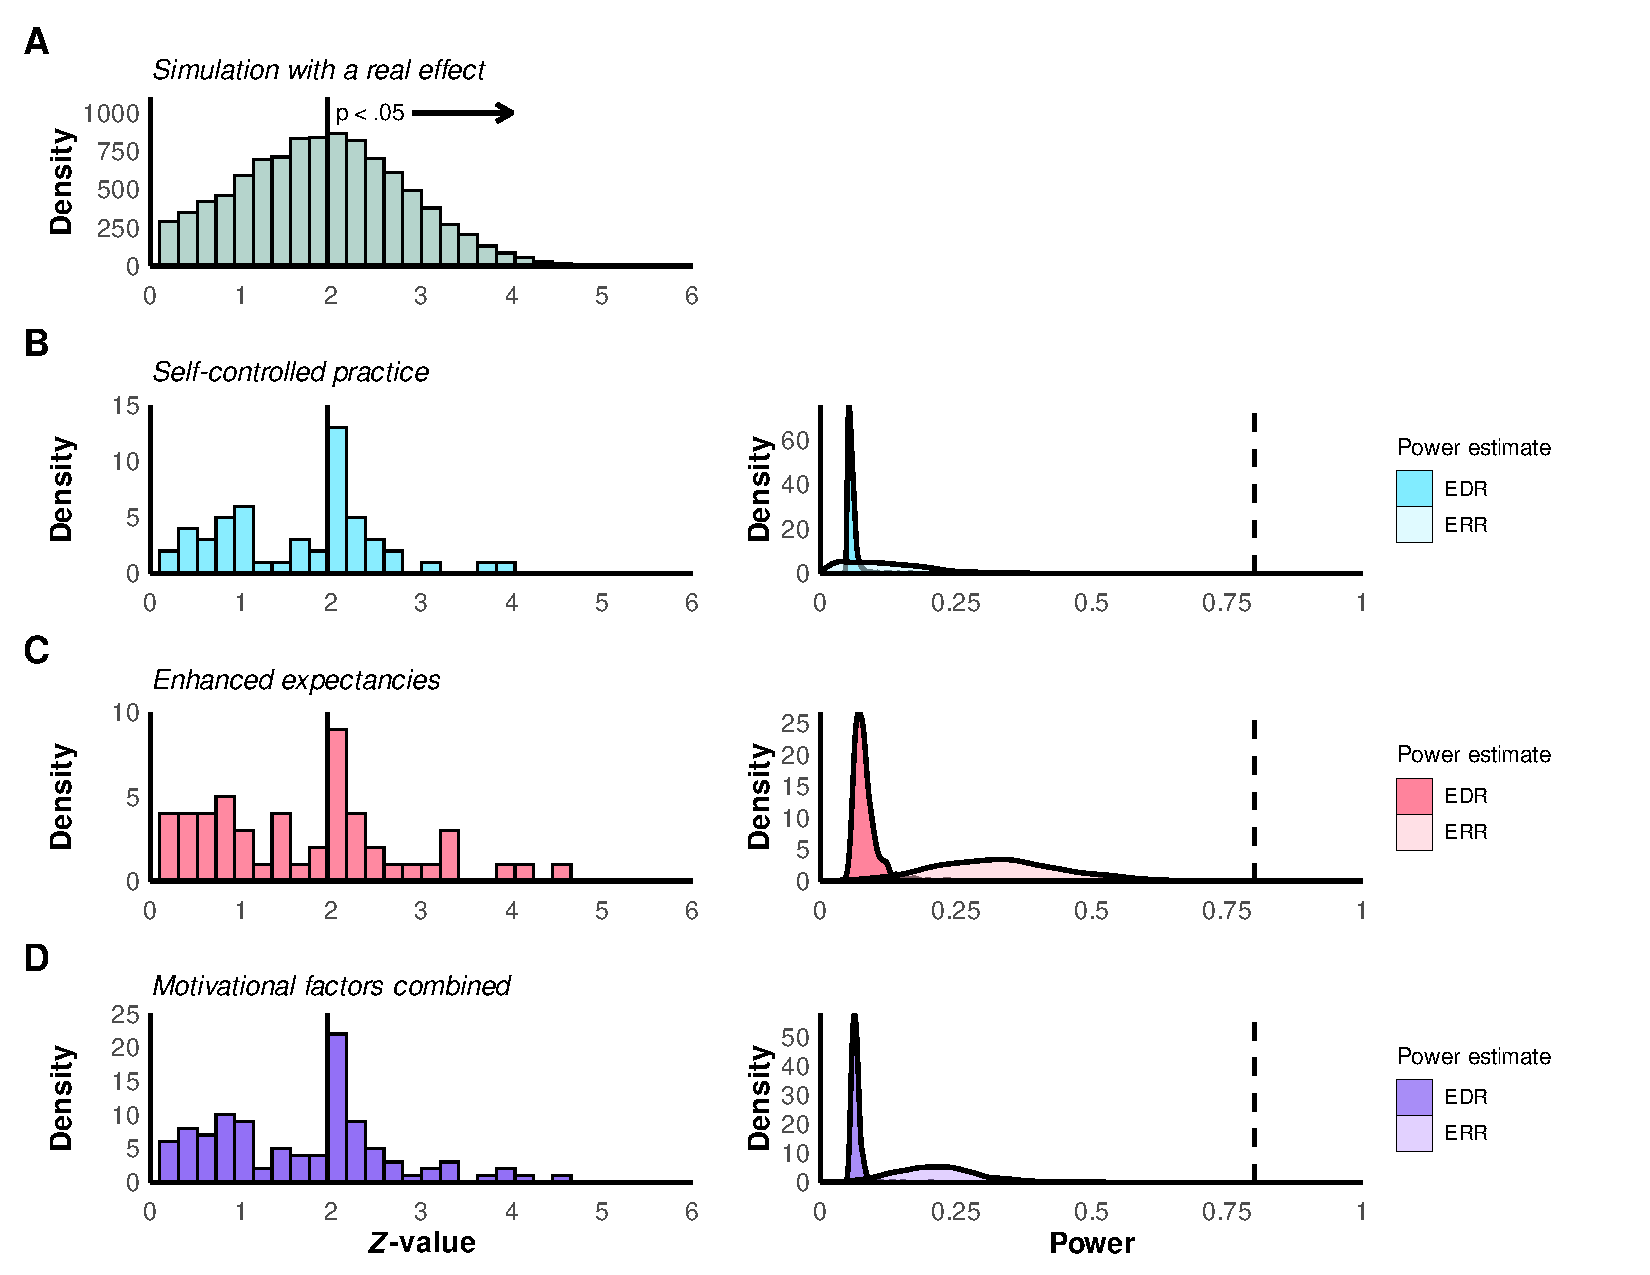
\includegraphics{../../figs/fig2} 

}

\caption{\normalfont \small \textbf{Results from the robust Bayesian meta-analysis with publication selection model-averaging (RoBMA-PSMA) method.} \textbf{(A)} Prior spike and distribution (purple) with 50\% of prior probability density concentrated on the null hypothesis and 50\% reflecting plausible true effects with \emph{M} = 0 and \emph{SD} = 1. (The x-axis is truncated; the prior did include a small probability of effects larger than 1 and smaller than -1.) The model-averaged posterior distribution of the mean effect (Mu) of \textbf{(B)} self-controlled practice on motor learning (blue). The increased height of the spike at mu = 0 reflects increased belief in the null hypothesis. The remaining distribution reflects updated belief in the size and direction of a possible true effect. The mean estimate (\emph{M} = .034) for the posterior distribution is represented by the dashed vertical line. The model-averaged posterior distribution of the mean effect of \textbf{(C)} enhanced expectancies on motor learning (red). The decreased height of the spike at mu = 0 reflects decreased belief in the null hypothesis. The remaining distribution reflected updated belief in the size and direction of a possible true effect. The mean estimate (\emph{M} = .26) for the posterior distribution is represented by the dashed vertical line. The model-averaged posterior distribution generated from an analysis of \textbf{(D)} simulated data (green). In the simulation, 49 studies were sampled from a population with a true effect of mu = .54 and no reporting bias. The mean estimate (\emph{M} = .504) for the posterior is represented by the vertical dashed line. Outliers were not included in the self-controlled (\emph{n} = 2) and enhanced expectancies (\emph{n} = 2) models.}\label{fig:fig2}
\end{figure}



\clearpage

\normalfont

\hypertarget{z-curve-1}{%
\subsection{\texorpdfstring{\emph{Z}-curve}{Z-curve}}\label{z-curve-1}}

\hypertarget{self-controlled-practice-1}{%
\subsubsection{Self-controlled practice}\label{self-controlled-practice-1}}

The results of the \emph{z}-curve analysis can be seen in Figure \ref{fig:fig3}B. The analysis estimated the average statistical power (expected discovery rate) of all experiments examining the effect of self-controlled practice was 6\% (95\% confidence intervals {[}5\%, 12\%{]}). Since the upper bound of the expected discovery rate does not overlap with the observed discovery rate of 48\% (95\% confidence interval {[}35\%, 62\%{]}), there is evidence of significant reporting bias. The estimated conditional power of the statistically significant results (expected replication rate) was 11\% (95\% confidence interval {[}3\%, 30\%{]}). Including influential cases did not markedly change the results.

\hypertarget{enhanced-expectancies-1}{%
\subsubsection{Enhanced expectancies}\label{enhanced-expectancies-1}}

The results of the \emph{z}-curve analysis can be seen in Figure \ref{fig:fig2}C. The analysis estimated that the expected discovery rate of studies conducted on enhanced expectancies was 8\% (95\% confidence interval {[}5\%, 18\%{]}). The observed discovery rate was 44\% (95\% confidence interval {[}31\%, 59\%{]}). Since the upper bound of the expected discovery rate does not overlap with the lower bound of the observed discovery rate, there is evidence of significant reporting bias. The expected replication rate of the statistically significant results was 33\% (95\% confidence interval {[}8\%, 59\%{]}). Including influential cases did not meaningfully change the results.

\hypertarget{motivational-factors-in-optimal-theory}{%
\subsubsection{Motivational factors in OPTIMAL theory}\label{motivational-factors-in-optimal-theory}}

The results of the \emph{z}-curve analysis of enhanced expectancy and self-controlled practice meta-data combined can be seen in Figure \ref{fig:fig3}D. The expected discovery rate of all studies conducted on the motivational factors in OPTIMAL theory is 6\% (95\% confidence interval {[}5\%, 13\%{]}). The observed discovery rate was 46\% (95\% confidence interval {[}37\%, 56\%{]}). The lower bound of the observed discovery rate does not overlap with the upper bound of the expected discovery rate, providing evidence of significant reporting bias in this literature. The expected replication rate of the statistically significant results was 21\% (95\% confidence interval {[}4\%, 39\%{]}). Including influential cases did not meaningfully change the results.

\clearpage

\begin{figure}

{\centering 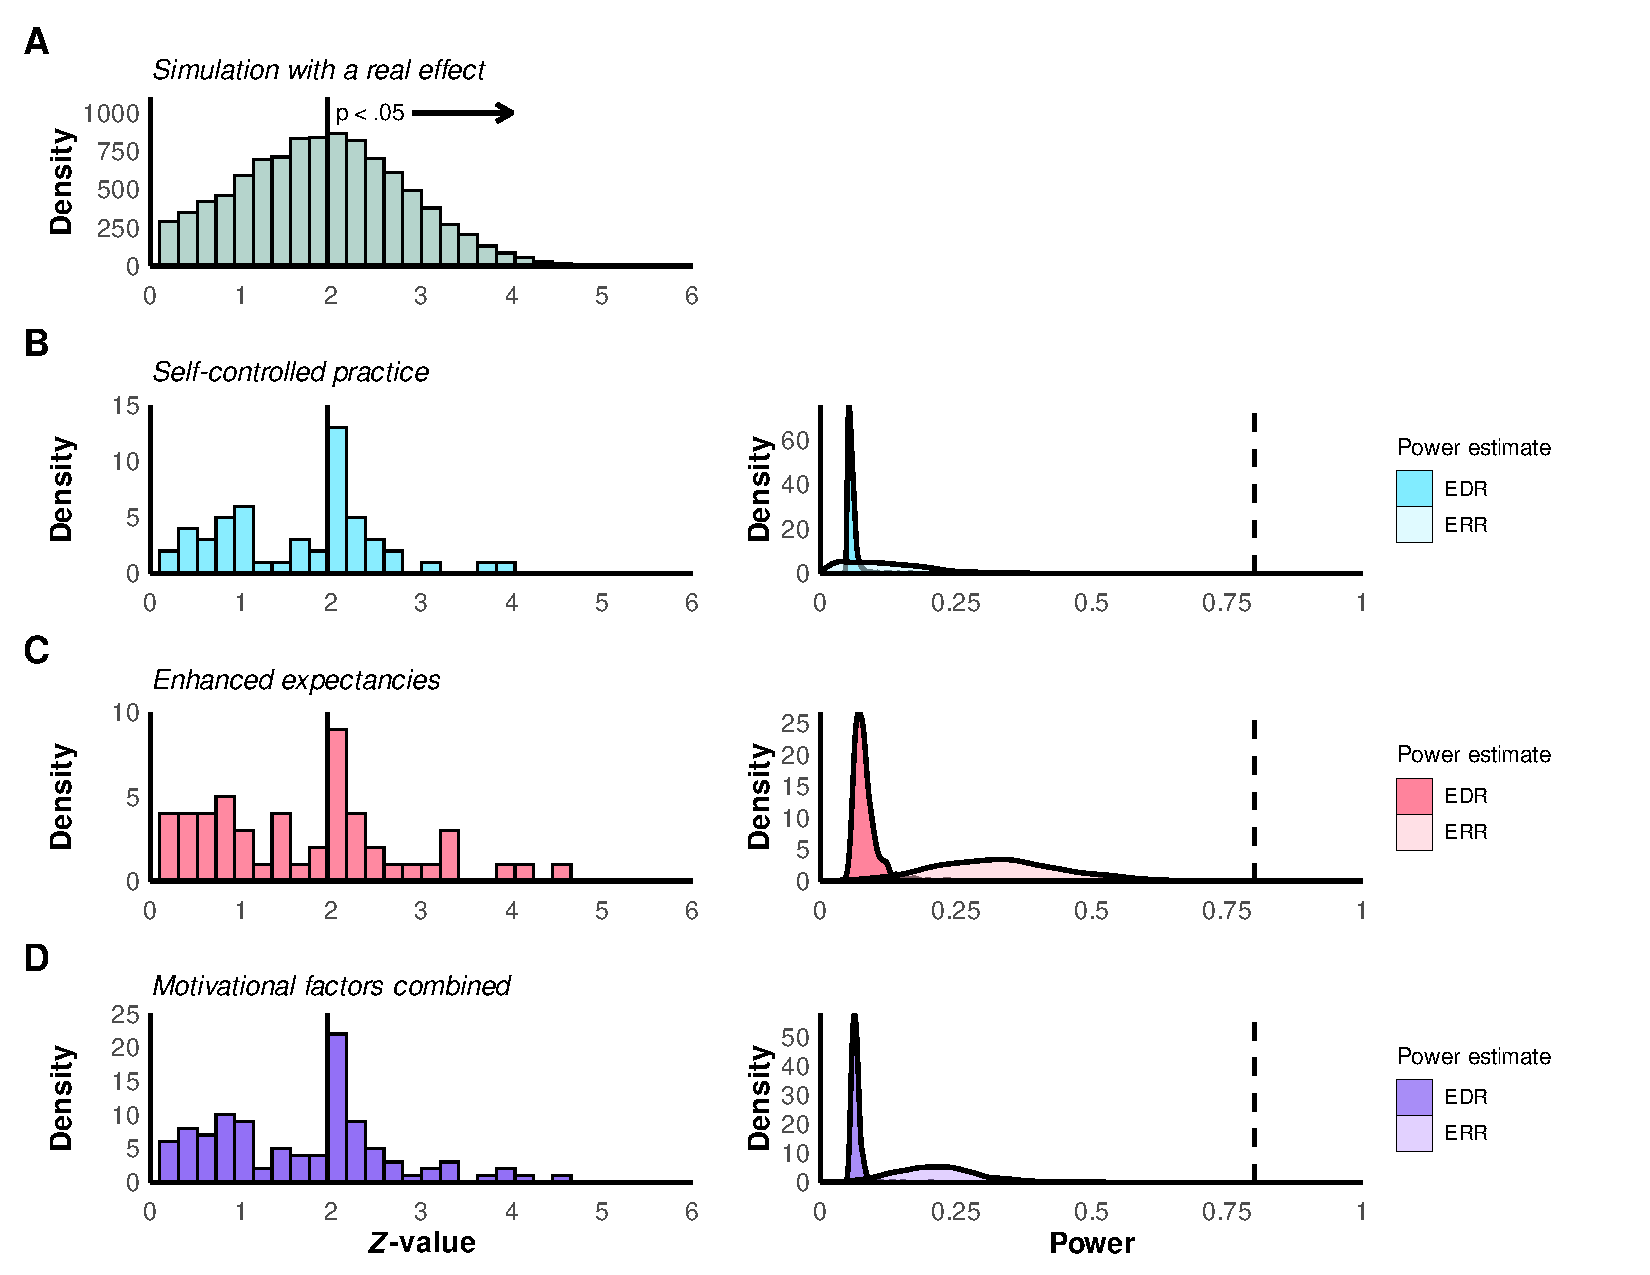
\includegraphics{../../figs/fig3} 

}

\caption{\normalfont \small \textbf{Results of the \emph{z}-curve analyses.} Distribution of \emph{z}-values for \textbf{(A)} our simulation with 47\% results and no reporting bias (green), \textbf{(B, left)} self-controlled practice (blue), \textbf{(C, left)} enhanced expectancies (red), and \textbf{(D, left)} motivational factors combined (purple). Values in the \emph{z}-score distributions for each analysis that are to the right of the significance line (\emph{z} = 1.96; solid, black) are statistically significant with a two-tailed \(\alpha\) of .05. Bootstrapped confidence distributions for the expected discovery rate (EDR; dark) and expected replication rate (ERR; light) for \textbf{(B, right)} self-controlled practice (blue), \textbf{(C, right)} enhanced expectancies (red), and \textbf{(D, right)} motivational factors combined (purple). Note, reported CIs include 5 extra points (EDR) and 3 extra points (ERR) added to the quantiles of the bootstrapped distributions in the right panel, consistent with Bartoš et al. (2022). The expected discovery rate is the estimated average power of all studies that have been conducted . The expected replication rate is the estimated power of all studies that observed a statistically significant result. The analysis estimated the average statistical power to be 6\%, 8\%, and 6\% for self-controlled practice, enhanced expectancies, and motivational factors combined, respectively. The estimated conditional power of the statistically significant results was 11\%, 33\%, and 21\% for self-controlled practice, enhanced expectancies, and motivational factors combined, respectively. Note that a minimum power of 80\% (dashed line, black) is often recommended. Outliers were not included in the self-controlled (\emph{n} = 2), enhanced expectancies (\emph{n} = 2), and motivational factors combined (\emph{n} = 4) analyses.}\label{fig:fig3}
\end{figure}



\clearpage

\normalsize

\hypertarget{discussion}{%
\section{Discussion}\label{discussion}}

A theory is formed based on observations of study results and/or real-world phenomena. It is evaluated by subsequent studies testing hypotheses derived from the theory. Thus, a theory's basis and support depend on the evidential value of the relevant studies. The OPTIMAL theory of motor learning (Wulf \& Lewthwaite, 2016) was established through study results showing that enhancing learners' expectancies and control over practice conditions improves learning and further supported by studies testing these hypotheses (Wulf \& Lewthwaite, 2021). Two recent meta-analyses were conducted to appraise the evidential value of studies testing whether self-controlled practice (McKay et al., in-press) and/or enhanced expectancies (Bacelar, Parma, Murrah, et al., 2022) improve motor learning. McKay and colleagues' (in-press) meta-analysis found self-controlled practice benefited motor learning (\emph{g} = 0.54) when using a naive random-effects model of published studies, but little evidence for a benefit was observed when a suite of bias correction techniques were employed (\emph{g}'s ranged from -0.11 to 0.26). McKay et al.~also used a \emph{z}-curve analysis to estimate the statistical power of self-controlled practice studies and found them to be severely underpowered (power = 6\%, 95\% confidence interval {[}5\%, 13\%{]}). Bacelar and colleagues' (2022) meta-analysis found evidence that enhanced expectancies improve motor learning when utilizing a naive random-effects model (\emph{g} = 0.54). Despite evidence of bias (i.e., funnel plot asymmetry), applying a trim-and-fill bias correction technique did not change the naive random-effects model estimate. Crucially, however, the trim-and-fill bias correction technique only slightly reduces bias and Type I error (Carter et al., 2019). Bacelar et al.~did not estimate the statistical power of enhanced expectancies studies; although they did note that the included studies had small sample sizes.

Our objective in the current study was to conduct a holistic assessment of the motivation pillar of OPTIMAL theory. Specifically, we used RoBMA-PSMA---a state-of-the-art bias correction technique---to evaluate the effect of self-controlled practice and enhanced expectancies on motor learning (see Figure \ref{fig:fig1}). Additionally, we used \emph{z}-curve analyses to estimate the statistical power of the enhanced expectancies studies alone and then combined with the self-controlled practice studies to assess the motivation pillar of OPTIMAL theory (see Figure \ref{fig:fig2}). Using RoBMA-PSMA to model the effect of self-controlled practice on motor learning, we found moderate evidence against the presence of an effect (BF\textsubscript{01} = 3.16). The model ensemble estimated a small average effect of \emph{d} = .034 with a 95\% credible interval that reached zero {[}.0, .248{]}. We also found overwhelming evidence for the presence of reporting bias (BF\textsubscript{pb} = 18,399). When modeling the effect of enhanced expectancies on motor learning with RoBMA-PSMA, we found weak evidence for the presence of an effect (BF\textsubscript{10} = 1.9). The model ensemble estimated a small average effect of \emph{d} = .26 with a 95\% credible interval that included zero {[}-.07, .63{]}. Weak evidence for the presence of reporting bias (BF\textsubscript{pb} = 2.3) was also found. There was very strong support for the presence of heterogeneity in the enhanced expectancies literature (BF\textsubscript{rf} = 47.6).

Heterogeneity can be problematic for modeling reporting bias with the selection and regression models employed in RoBMA-PSMA (Carter et al., 2019). Fortunately, the \emph{z}-curve was designed for heterogeneous samples and may therefore be a better method of evaluating reporting bias in the enhanced expectancies data. The \emph{z}-curve analysis estimated the average statistical power of enhanced expectancies studies to be 8\%. The 95\% confidence interval {[}5\%, 18\%{]} did not overlap with the 95\% confidence interval of the observed discovery rate {[}31\%, 59\%{]}, providing evidence of significant reporting bias. Visual inspection of the distribution of \emph{z}-values reveals a large concentration of barely significant results and a dearth of barely not significant results (Figure \ref{fig:fig2}B). This pattern is consistent with selective reporting, and it is difficult to imagine an alternate process that would generate these results. To evaluate the potential presence of reporting bias across both motivation factors, as well as estimate the average power of studies that have investigated these phenomena, we applied a \emph{z}-curve to studies from both meta-analyses. The \emph{z}-curve analysis combining the enhanced expectancies and self-controlled practice studies estimated the average statistical power to be 6\%. The 95\% confidence interval {[}5\%, 13\%{]} did not overlap with the 95\% confidence interval of the observed discovery rate {[}37\%, 56\%{]}, indicating significant reporting bias.

Our results are mostly consistent with other recent meta-analyses and pre-registered experiments with large sample sizes that have raised concerns about the state of evidence for the motivation pillar in OPTIMAL theory. Concerning self-controlled practice, the RoBMA-PSMA estimate of \emph{d} =.034 is within the range of estimates reported by McKay et al. (in-press), which showed \emph{g}'s ranging from -0.11 to 0.26. Our finding of overwhelming evidence for reporting bias is also consistent with McKay and colleagues' \emph{z}-curve showing the 95\% confidence interval for average statistical power was 5\% to 13\% and an observed discovery rate of 37\% to 56\%. Four recent pre-registered studies with relatively large sample sizes have all failed to observe a self-controlled practice or learning benefit (Bacelar, Parma, Cabral, et al., 2022; McKay \& Ste-Marie, 2022; St. Germain et al., 2022; Yantha et al., 2022). For example, Bacelar, Parma, Cabral, et al. (2022) had 100 participants practice a non-dominant arm bean bag tossing task with self-controlled augmented knowledge of results feedback and 100 participants practice the task without choice, and did not find a self-controlled learning advantage. Regarding enhanced expectancies, our RoMBA-PSMA estimate of \emph{d} = 0.26 is consistent with Bacelar and colleagues' (2022) concern that their meta-analysis yielded an overestimated effect size (\emph{g} = 0.54). Likewise, our \emph{z}-curve result that enhanced expectancies are underpowered and subject to reporting bias is consistent with Bacelar and colleagues' findings of small sample sizes (median = 14/group) and small-study effects (i.e., significant funnel plot asymmetry). Estimates of reporting bias from the RoBMA-PSMA models were sensitive to the removal of two outliers, showing strong support for bias only when one or two outliers were included but not when both were removed. The evidence of reporting bias observed in the \emph{z}-curve was not sensitive to removal of outliers and with the heterogeneity in the sample the \emph{z}-curve may provide a better test of bias than RoBMA-PSMA. Considering these motivational factors combined, the \emph{z}-curve result that studies supporting OPTIMAL theory are underpowered and subject to reporting bias is consistent with McKay and colleagues' (in-press) meta-analysis that drew the same conclusion about self-controlled practice studies. Taken together, past and present results suggest that the our samples of studies demonstrating the benefit of enhancing learners' expectancies and giving them control over practice conditions presents a distorted reality due to reporting bias. These effects are not reliably different from zero, highlighting that the motivation pillar of OPTIMAL theory lacks evidential value.

\hypertarget{limitations}{%
\subsection{Limitations}\label{limitations}}

Our efforts to model selective reporting and adjust our parameter estimates accordingly are limited by the difficult nature of this task. We simply cannot know the extent of reporting bias in the extant literature, nor can we know the underlying mechanisms responsible for it. While our models correspond nicely to plausible selection processes, there are other possible mechanisms that could cause the data to fit our bias-correction models. For instance, it is possible researchers were able to intuit the size of the effects they would observe with their specific sample and paradigm, and they carefully adjusted their sample sizes based on these intuitions. If this was the case, we would expect large studies for small effects and small studies for large ones, consistent with the regression models included in the RoBMA-PSMA. Although we consider this unlikely---how could researchers have such a fine-grained understanding of the effects they are studying given the uncertainty in the literature?---the reader should be aware of the sensitivity of our models to assumptions about the underlying data generating process. The likely presence of heterogeneity in the enhanced expectancies literature suggests there is not one true effect, so individual studies may have been testing interventions with real benefits. However, this also means individual studies may have been testing interventions with real detriments as well, and we cannot discern which studies fall into which category.

\hypertarget{conclusion}{%
\section{Conclusion}\label{conclusion}}

Our analyses suggest a lack of evidence in support of enhanced expectancies and self-controlled practice as beneficial motor learning interventions. The lack of evidence supporting the motivational branch in OPTIMAL theory is not evidence that the predicted effects are absent. Indeed, even the null effects for a self-controlled practice benefit reported by pre-registered studies with large sample sizes (Bacelar, Parma, Cabral, et al., 2022; McKay \& Ste-Marie, 2022; St. Germain et al., 2022; Yantha et al., 2022) are not conclusive that an effect is absent. Rather, these null effects leave open the possibility that the effect is very small and, thus, not detectable even with relatively large sample sizes (e.g., \emph{N} = 200 as in Bacelar, Parma, Cabral, et al. (2022)). Motor learning researchers often study skills performed in sports, which are often \emph{games of inches}, so very small effects may be of practical interest. Nonetheless, the field of motor learning is not past asking whether self-controlled practice and enhanced expectancies have any benefit, so concerns about estimating the magnitude of a potential benefit are premature (Simonsohn, 2015). Thus, we urge any motor learning scientist(s) interested in clarifying whether self-controlled practice or enhanced expectancies boost motor learning to address the problems of underpowered and overworked study designs (Lohse et al., 2016) and the reporting bias revealed in the present meta-analysis and those by McKay et al. (in-press) and Bacelar, Parma, Murrah, et al. (2022).

There are multiple ways to increase statistical power, such as accounting for between-subjects variance by using a covariate, like pretest motor performance, in an ANCOVA design (Vickers \& Altman, 2001), and/or increasing the number of pretest and posttest trials (Maxwell et al., 1991). Perhaps the most common and effective way to boost power is to increase sample size. Lakens (2022) describes several approaches for determining sample size, including conducting an \emph{a priori} power analysis. A recent survey of three popular motor learning journals revealed a low prevalence (84/635 or 13\% in McKay, Corson, et al., 2022) and low reproducibility (7/84 or 8\% in McKay, Bacelar, et al., 2022) of reported \emph{a priori} power analyses. The usefulness of an \emph{a priori} power analysis depends on reasonable assumptions about effect sizes. Assumptions about the effect size for self-controlled practice and enhanced expectancies studies should be based on the bias-corrected estimates found in the present study (self-controlled practice: \emph{d} = .034; enhanced expectancies: \emph{d} = 0.26) given the evidence of reporting bias. Researchers could also use the smallest effect size of interest (Lakens, 2022), but this effect may be even smaller than those from the meta-analyses, as noted earlier. Simonsohn (2015) described another approach to determine sample size for replication studies termed the ``small telescopes'' approach. This approach recommends the replication sample size be 2.5 times that of the original sample. With questions surrounding the face value of original studies supporting OPTIMAL theory, we believe replication studies are crucial and the ``small telescopes'' approach to determine sample size for these studies should be the minimally accepted approach. Irrespective of which of the above approaches researchers use to make reasonable assumptions about effect sizes, their \emph{a priori} power analyses will likely lead to sample sizes that are larger than they are used to collecting. Thus, researchers may want to consider ways to improve the efficiency of their data collection, for example by using sequential analyses (Lakens et al., 2021; Lakens, 2014; Wald, 1945) or conducting multi-laboratory studies. Finally, clarity about the effect of self-controlled practice and/or enhanced expectancies on motor learning can only be achieved if a complete picture of the evidence is available. Researchers and gatekeepers to scientific publication (e.g., peer-reviewers, journal editors) should take measures to eliminate reporting bias, for example by publishing registered reports, undertaking/encouraging replication attempts (at a minimum using the ``small telescopes'' approach), and publishing null effects.

\vfill

\hypertarget{author-contributions-credit-taxonomy}{%
\subsection{Author Contributions (CRediT Taxonomy)}\label{author-contributions-credit-taxonomy}}

\noindent Conceptualization: BM, MFBB, JOP, MWM, MJC\\
Data curation: BM, MJC\\
Formal analysis: BM\\
Funding acquisition: MJC\\
Investigation: BM, MFBB, JOP, MWM, MJC\\
Methodology: BM, MFBB, JOP, MWM, MJC\\
Project administration: BM, MFBB, JOP, MWM, MJC\\
Software: BM, MJC\\
Supervision: MWM, MJC\\
Validation: BM, MJC\\
Visualization: BM, MJC\\
Writing -- original draft: BM, MFBB, JOP, MWM, MJC\\
Writing -- review \& editing: BM, MFBB, JOP, MWM, MJC

\hypertarget{acknowledgements}{%
\subsection{Acknowledgements}\label{acknowledgements}}

\noindent The first and last author would like to thank František Bartoš for drawing their attention to the \texttt{RoBMA} package during the review of the original self-controlled learning meta-analysis and for providing helpful feedback on an earlier draft of this manuscript.

\hypertarget{open-science-practices}{%
\subsection{Open Science Practices}\label{open-science-practices}}

\noindent The data and scripts can be accessed using either of the following links: \url{https://osf.io/vfza7/} or \url{https://github.com/cartermaclab/proj_sc-ee-optimal-theory}

\hypertarget{conflicts-of-interest}{%
\subsection{Conflicts of Interest}\label{conflicts-of-interest}}

\noindent All authors declare no conflicts of interest.

\hypertarget{funding}{%
\subsection{Funding}\label{funding}}

\noindent This work was supported by the Natural Sciences and Engineering Research Council (NSERC) of Canada (RGPIN-2018-05589; MJC) and McMaster University (MJC).

\hypertarget{references}{%
\section{References}\label{references}}

\vspace{2ex}

\hypertarget{refs}{}
\begin{CSLReferences}{1}{0}
\leavevmode\vadjust pre{\hypertarget{ref-abe2011}{}}%
Abe, M., Schambra, H., Wassermann, E. M., Luckenbaugh, D., Schweighofer, N., \& Cohen, L. G. (2011). Reward improves long-term retention of a motor memory through induction of offline memory gains. \emph{Current Biology}, \emph{21}(7), 557--562. \url{https://doi.org/10.1016/j.cub.2011.02.030}

\leavevmode\vadjust pre{\hypertarget{ref-R-papaja}{}}%
Aust, F., \& Barth, M. (2020). \emph{{papaja}: {Prepare} reproducible {APA} journal articles with {R Markdown}}. \url{https://github.com/crsh/papaja}

\leavevmode\vadjust pre{\hypertarget{ref-avila2012}{}}%
Ávila, L. T. G., Chiviacowsky, S., Wulf, G., \& Lewthwaite, R. (2012). Positive social-comparative feedback enhances motor learning in children. \emph{Psychology of Sport and Exercise}, \emph{13}(6), 849--853. \url{https://doi.org/10.1016/j.psychsport.2012.07.001}

\leavevmode\vadjust pre{\hypertarget{ref-bacelar2022a}{}}%
Bacelar, M. F. B., Parma, J. O., Cabral, D., Daou, M., Lohse, K. R., \& Miller, M. W. (2022). Dissociating the contributions of motivational and information processing factors to the self-controlled feedback learning benefit. \emph{Psychology of Sport and Exercise}, \emph{59}, 102119. \url{https://doi.org/10.1016/j.psychsport.2021.102119}

\leavevmode\vadjust pre{\hypertarget{ref-bacelar2022}{}}%
Bacelar, M. F. B., Parma, J. O., Murrah, W. M., \& Miller, M. W. (2022). Meta-analyzing enhanced expectancies on motor learning: Positive effects but methodological concerns. \emph{International Review of Sport and Exercise Psychology}, \emph{0}(0), 1--30. \url{https://doi.org/10.1080/1750984X.2022.2042839}

\leavevmode\vadjust pre{\hypertarget{ref-R-tinylabels}{}}%
Barth, M. (2022). \emph{{tinylabels}: Lightweight variable labels}. \url{https://cran.r-project.org/package=tinylabels}

\leavevmode\vadjust pre{\hypertarget{ref-R-robma}{}}%
Bartoš, F., \& Maier, M. (2020). \emph{RoBMA: An r package for robust bayesian meta-analyses}. \url{https://CRAN.R-project.org/package=RoBMA}

\leavevmode\vadjust pre{\hypertarget{ref-bartos2021}{}}%
Bartoš, F., Maier, M., Wagenmakers, E.-J., Doucouliagos, H., \& Stanley, T. D. (2022). Robust bayesian meta-analysis: Model-averaging across complementary publication bias adjustment methods. \emph{Research Synthesis Methods}, 1--18. \url{https://doi.org/10.1002/jrsm.1594}

\leavevmode\vadjust pre{\hypertarget{ref-R-zcurve}{}}%
Bartoš, F., \& Schimmack, U. (2020). \emph{Zcurve: An r package for fitting z-curves}. \url{https://CRAN.R-project.org/package=zcurve}

\leavevmode\vadjust pre{\hypertarget{ref-bartos2020}{}}%
Bartoš, F., \& Schimmack, U. (in-press). Z-curve 2.0: Estimating replication rates and discovery rates. \emph{Meta-Psychology}. \url{https://doi.org/10.31234/osf.io/urgtn}

\leavevmode\vadjust pre{\hypertarget{ref-R-geomtextpath}{}}%
Cameron, A., \& van den Brand, T. (2022). \emph{Geomtextpath: Curved text in 'ggplot2'}. \url{https://CRAN.R-project.org/package=geomtextpath}

\leavevmode\vadjust pre{\hypertarget{ref-carter2019}{}}%
Carter, E. C., Schönbrodt, F. D., Gervais, W. M., \& Hilgard, J. (2019). Correcting for bias in psychology: A comparison of meta-analytic methods. \emph{Advances in Methods and Practices in Psychological Science}, \emph{2}(2), 115--144. \url{https://doi.org/10.1177/2515245919847196}

\leavevmode\vadjust pre{\hypertarget{ref-R-pwr}{}}%
Champely, S. (2020). \emph{Pwr: Basic functions for power analysis}. \url{https://CRAN.R-project.org/package=pwr}

\leavevmode\vadjust pre{\hypertarget{ref-chiviacowsky2007}{}}%
Chiviacowsky, S., \& Wulf, G. (2007). Feedback after good trials enhances learning. \emph{Research Quarterly for Exercise and Sport}, \emph{78}(2), 40--47. \url{https://doi.org/10.1080/02701367.2007.10599402}

\leavevmode\vadjust pre{\hypertarget{ref-cimpian2007}{}}%
Cimpian, A., Arce, H.-M. C., Markman, E. M., \& Dweck, C. S. (2007). Subtle linguistic cues affect children's motivation. \emph{Psychological Science}, \emph{18}(4), 314--316. \url{https://doi.org/10.1111/j.1467-9280.2007.01896.x}

\leavevmode\vadjust pre{\hypertarget{ref-osc2015}{}}%
Collaboration, O. S. (2015). Estimating the reproducibility of psychological science. \emph{Science}, \emph{349}(6251), 943--943. \url{https://www.jstor.org/stable/24749235}

\leavevmode\vadjust pre{\hypertarget{ref-dempster1977}{}}%
Dempster, A. P., Laird, N. M., \& Rubin, D. B. (1977). Maximum likelihood from incomplete data via the {EM} algorithm. \emph{Journal of the Royal Statistical Society. Series B (Methodological)}, \emph{39}(1), 1--38. \url{https://www.jstor.org/stable/2984875}

\leavevmode\vadjust pre{\hypertarget{ref-duval1998}{}}%
Duval, S., \& Tweedie, R. (1998). Practical estimates of the effect of publication bias in meta-analysis. \emph{Australasian Epidemiologist}, \emph{5}(4). \url{https://doi.org/10.3316/informit.434005834350149}

\leavevmode\vadjust pre{\hypertarget{ref-fanelli2010}{}}%
Fanelli, D. (2010). Do pressures to publish increase scientists' bias? An empirical support from US states data. \emph{PLOS ONE}, \emph{5}(4), e10271. \url{https://doi.org/10.1371/journal.pone.0010271}

\leavevmode\vadjust pre{\hypertarget{ref-gelman2014}{}}%
Gelman, A., \& Carlin, J. (2014). Beyond power calculations: {Assessing Type S} (sign) and {Type M} (magnitude) errors. \emph{Perspectives on Psychological Science}, \emph{9}(6), 641--651. \url{https://doi.org/10.1177/1745691614551642}

\leavevmode\vadjust pre{\hypertarget{ref-guadagnoli2004}{}}%
Guadagnoli, M. A., \& Lee, T. D. (2004). Challenge point: A framework for conceptualizing the effects of various practice conditions in motor learning. \emph{Journal of Motor Behavior}, \emph{36}(2), 212--224. \url{https://doi.org/10.3200/JMBR.36.2.212-224}

\leavevmode\vadjust pre{\hypertarget{ref-hagger2016}{}}%
Hagger, M. S., Chatzisarantis, N. L. D., Alberts, H., Anggono, C. O., Batailler, C., Birt, A. R., Brand, R., Brandt, M. J., Brewer, G., Bruyneel, S., Calvillo, D. P., Campbell, W. K., Cannon, P. R., Carlucci, M., Carruth, N. P., Cheung, T., Crowell, A., De Ridder, D. T. D., Dewitte, S., \ldots{} Zwienenberg, M. (2016). A multilab preregistered replication of the ego-depletion effect. \emph{Perspectives on Psychological Science}, \emph{11}(4), 546--573. \url{https://doi.org/10.1177/1745691616652873}

\leavevmode\vadjust pre{\hypertarget{ref-R-gt}{}}%
Iannone, R., Cheng, J., \& Schloerke, B. (2022). \emph{Gt: Easily create presentation-ready display tables}. \url{https://CRAN.R-project.org/package=gt}

\leavevmode\vadjust pre{\hypertarget{ref-R-invgamma}{}}%
Kahle, D., \& Stamey, J. (2017). \emph{Invgamma: The inverse gamma distribution}. \url{https://CRAN.R-project.org/package=invgamma}

\leavevmode\vadjust pre{\hypertarget{ref-lakens2014}{}}%
Lakens, D. (2014). Performing high-powered studies efficiently with sequential analyses. \emph{European Journal of Social Psychology}, \emph{44}(7), 701--710. \url{https://doi.org/10.1002/ejsp.2023}

\leavevmode\vadjust pre{\hypertarget{ref-lakens2022}{}}%
Lakens, D. (2022). Sample size justification. \emph{Collabra: Psychology}, \emph{8}(1), 33267. \url{https://doi.org/10.1525/collabra.33267}

\leavevmode\vadjust pre{\hypertarget{ref-lakens2021}{}}%
Lakens, D., Pahlke, F., \& Wassmer, G. (2021). \emph{Group sequential designs: A tutorial}. {PsyArXiv}. \url{https://doi.org/10.31234/osf.io/x4azm}

\leavevmode\vadjust pre{\hypertarget{ref-lee2011}{}}%
Lee, C., Linkenauger, S. A., Bakdash, J. Z., Joy-Gaba, J. A., \& Profitt, D. R. (2011). Putting like a pro: The role of positive contagion in golf performance and perception. \emph{PLOS ONE}, \emph{6}(10), e26016. \url{https://doi.org/10.1371/journal.pone.0026016}

\leavevmode\vadjust pre{\hypertarget{ref-lee2012}{}}%
Lee, G., \& Scott, C. (2012). {EM} algorithms for multivariate {Gaussian} mixture models with truncated and censored data. \emph{Computational Statistics \& Data Analysis}, \emph{56}(9), 2816--2829. \url{https://doi.org/10.1016/j.csda.2012.03.003}

\leavevmode\vadjust pre{\hypertarget{ref-lee2021}{}}%
Lee, T. D., \& Carnahan, H. (2021). Motor learning: Reflections on the past 40 years of research. \emph{Kinesiology Review}, \emph{10}(3), 274--282. \url{https://doi.org/10.1123/kr.2021-0018}

\leavevmode\vadjust pre{\hypertarget{ref-lewthwaite2015}{}}%
Lewthwaite, R., Chiviacowsky, S., Drews, R., \& Wulf, G. (2015). Choose to move: The motivational impact of autonomy support on motor learning. \emph{Psychonomic Bulletin \& Review}, \emph{22}(5), 1383--1388. \url{https://doi.org/10.3758/s13423-015-0814-7}

\leavevmode\vadjust pre{\hypertarget{ref-lohse2016}{}}%
Lohse, K., Buchanan, T., \& Miller, M. (2016). Underpowered and overworked: Problems with data analysis in motor learning studies. \emph{Journal of Motor Learning and Development}, \emph{4}(1), 37--58. \url{https://doi.org/10.1123/jmld.2015-0010}

\leavevmode\vadjust pre{\hypertarget{ref-maier2022}{}}%
Maier, M., Bartoš, F., \& Wagenmakers, E.-J. (in-press). Robust {Bayesian} meta-analysis: Addressing publication bias with model-averaging. \emph{Psychological Methods}. \url{https://doi.org/10.1037/met0000405}

\leavevmode\vadjust pre{\hypertarget{ref-mathur2020}{}}%
Mathur, M. B., \& VanderWeele, T. J. (2020). Sensitivity analysis for publication bias in meta-analyses. \emph{Journal of the Royal Statistical Society: Series C (Applied Statistics)}, \emph{69}(5), 1091--1119. \url{https://doi.org/10.1111/rssc.12440}

\leavevmode\vadjust pre{\hypertarget{ref-maxwell1991}{}}%
Maxwell, S. E., Cole, D. A., Arvey, R. D., \& Salas, E. (1991). A comparison of methods for increasing power in randomized between-subjects designs. \emph{Psychological Bulletin}, \emph{110}(2), 328--337. \url{https://doi.org/10.1037/0033-2909.110.2.328}

\leavevmode\vadjust pre{\hypertarget{ref-mckay2022c}{}}%
McKay, B., Bacelar, M. F. B., \& Carter, M. J. (2022). \emph{\href{}{On the reproducibility of power analyses in motor behavior research}}. {SportRxiv}.

\leavevmode\vadjust pre{\hypertarget{ref-mckay2022b}{}}%
McKay, B., Corson, A., Vinh, M.-A., Jeyarajan, G., Tandon, C., Brooks, H., Hubley, J., \& Carter, M. J. (2022). \emph{Low prevalence of a priori power analyses in motor behavior research}. {SportRxiv}. \url{https://doi.org/10.51224/SRXIV.175}

\leavevmode\vadjust pre{\hypertarget{ref-mckay2022}{}}%
McKay, B., \& Ste-Marie, D. M. (2022). Autonomy support via instructionally irrelevant choice not beneficial for motor performance or learning. \emph{Research Quarterly for Exercise and Sport}, \emph{93}(1), 64--76. \url{https://doi.org/10.1080/02701367.2020.1795056}

\leavevmode\vadjust pre{\hypertarget{ref-mckay2021}{}}%
McKay, B., Yantha, Z. D., Hussien, J., Carter, M. J., \& Ste-Marie, D. M. (in-press). Meta-analytic findings in the self-controlled motor learning literature: Underpowered, biased, and lacking evidential value. \emph{Meta-Psychology}. \url{https://doi.org/10.31234/osf.io/8d3nb}

\leavevmode\vadjust pre{\hypertarget{ref-mcshane2016}{}}%
McShane, B. B., Böckenholt, U., \& Hansen, K. T. (2016). Adjusting for publication bias in meta-analysis: An evaluation of selection methods and some cautionary notes. \emph{Perspectives on Psychological Science}, \emph{11}(5), 730--749. \url{https://doi.org/10.1177/1745691616662243}

\leavevmode\vadjust pre{\hypertarget{ref-munafo2017}{}}%
Munafò, M. R., Nosek, B. A., Bishop, D. V. M., Button, K. S., Chambers, C. D., Percie du Sert, N., Simonsohn, U., Wagenmakers, E.-J., Ware, J. J., \& Ioannidis, J. P. A. (2017). A manifesto for reproducible science. \emph{Nature Human Behaviour}, \emph{1}(1, 1), 1--9. \url{https://doi.org/10.1038/s41562-016-0021}

\leavevmode\vadjust pre{\hypertarget{ref-R-truncdist}{}}%
Novomestky, F., \& Nadarajah, S. (2016). \emph{Truncdist: Truncated random variables}. \url{https://CRAN.R-project.org/package=truncdist}

\leavevmode\vadjust pre{\hypertarget{ref-R-patchwork}{}}%
Pedersen, T. L. (2022). \emph{Patchwork: The composer of plots}.

\leavevmode\vadjust pre{\hypertarget{ref-R-base}{}}%
R Core Team. (2021). \emph{R: A language and environment for statistical computing}. R Foundation for Statistical Computing. \url{https://www.R-project.org/}

\leavevmode\vadjust pre{\hypertarget{ref-salmoni1984}{}}%
Salmoni, A. W., Schmidt, R. A., \& Walter, C. B. (1984). Knowledge of results and motor learning: A review and critical reappraisal. \emph{Psychological Bulletin}, \emph{95}(3), 355--386. \url{https://doi.org/10.1037/0033-2909.95.3.355}

\leavevmode\vadjust pre{\hypertarget{ref-sanli2013}{}}%
Sanli, E., Patterson, J., Bray, S., \& Lee, T. (2013). Understanding self-controlled motor learning protocols through the self-determination theory. \emph{Frontiers in Psychology}, \emph{3}. \url{https://www.frontiersin.org/articles/10.3389/fpsyg.2012.00611}

\leavevmode\vadjust pre{\hypertarget{ref-schmidt1975}{}}%
Schmidt, R. A. (1975). A schema theory of discrete motor skill learning. \emph{Psychological Review}, \emph{82}(4), 225--260. \url{https://doi.org/10.1037/h0076770}

\leavevmode\vadjust pre{\hypertarget{ref-R-plotly}{}}%
Sievert, C. (2020). \emph{Interactive web-based data visualization with r, plotly, and shiny}. Chapman; Hall/CRC. \url{https://plotly-r.com}

\leavevmode\vadjust pre{\hypertarget{ref-simonsohn2015}{}}%
Simonsohn, U. (2015). Small telescopes: Detectability and the evaluation of replication results. \emph{Psychological Science}, \emph{26}(5), 559--569. \url{https://doi.org/10.1177/0956797614567341}

\leavevmode\vadjust pre{\hypertarget{ref-stgermain2022}{}}%
St. Germain, L., Williams, A., Balbaa, N., Poskus, A., Lohse, K. R., \& Carter, M. J. (2022). Increased perceptions of autonomy through choice fail to enhance motor skill retention. \emph{Journal of Experimental Psychology: Human Perception and Performance}, \emph{48}(4), 370--379. \url{https://doi.org/10.1037/xhp0000992}

\leavevmode\vadjust pre{\hypertarget{ref-stefan2022}{}}%
Stefan, A., \& Schönbrodt, F. (2022). \emph{Big little lies: A compendium and simulation of p-hacking strategies}. {PsyArXiv}. \url{https://doi.org/10.31234/osf.io/xy2dk}

\leavevmode\vadjust pre{\hypertarget{ref-stemarie2011}{}}%
Ste-Marie, D., Vertes, K., Rymal, A., \& Martini, R. (2011). Feedforward self-modeling enhances skill acquisition in children learning trampoline skills. \emph{Frontiers in Psychology}, \emph{2}. \url{https://www.frontiersin.org/articles/10.3389/fpsyg.2011.00155}

\leavevmode\vadjust pre{\hypertarget{ref-sterne2000}{}}%
Sterne, J. A. C., Gavaghan, D., \& Egger, M. (2000). Publication and related bias in meta-analysis: Power of statistical tests and prevalence in the literature. \emph{Journal of Clinical Epidemiology}, \emph{53}(11), 1119--1129. \url{https://doi.org/10.1016/S0895-4356(00)00242-0}

\leavevmode\vadjust pre{\hypertarget{ref-sutton2000}{}}%
Sutton, A., Song, F., Gilbody, S., \& Abrams, K. (2000). Modelling publication bias in meta-analysis: A review. \emph{Statistical Methods in Medical Research}, \emph{9}(5), 421--445. \url{https://doi.org/10.1177/096228020000900503}

\leavevmode\vadjust pre{\hypertarget{ref-thornton2000}{}}%
Thornton, A., \& Lee, P. (2000). Publication bias in meta-analysis: Its causes and consequences. \emph{Journal of Clinical Epidemiology}, \emph{53}(2), 207--216. \url{https://doi.org/10.1016/S0895-4356(99)00161-4}

\leavevmode\vadjust pre{\hypertarget{ref-R-renv}{}}%
Ushey, K. (2022). \emph{Renv: Project environments}. \url{https://CRAN.R-project.org/package=renv}

\leavevmode\vadjust pre{\hypertarget{ref-vevea2005}{}}%
Vevea, J. L., \& Woods, C. M. (2005). Publication bias in research synthesis: Sensitivity analysis using a priori weight functions. \emph{Psychological Methods}, \emph{10}(4), 428--443. \url{https://doi.org/10.1037/1082-989X.10.4.428}

\leavevmode\vadjust pre{\hypertarget{ref-vickers2001}{}}%
Vickers, A. J., \& Altman, D. G. (2001). Analysing controlled trials with baseline and follow up measurements. \emph{BMJ}, \emph{323}(7321), 1123--1124. \url{https://doi.org/10.1136/bmj.323.7321.1123}

\leavevmode\vadjust pre{\hypertarget{ref-R-metafor}{}}%
Viechtbauer, W. (2010). Conducting meta-analyses in {R} with the {metafor} package. \emph{Journal of Statistical Software}, \emph{36}(3), 1--48. \url{https://doi.org/10.18637/jss.v036.i03}

\leavevmode\vadjust pre{\hypertarget{ref-wald1945}{}}%
Wald, A. (1945). Sequential tests of statistical hypotheses. \emph{The Annals of Mathematical Statistics}, \emph{16}(2), 117--186. \url{https://www.jstor.org/stable/2235829}

\leavevmode\vadjust pre{\hypertarget{ref-R-tidyverse}{}}%
Wickham, H., Averick, M., Bryan, J., Chang, W., McGowan, L. D., François, R., Grolemund, G., Hayes, A., Henry, L., Hester, J., Kuhn, M., Pedersen, T. L., Miller, E., Bache, S. M., Müller, K., Ooms, J., Robinson, D., Seidel, D. P., Spinu, V., \ldots{} Yutani, H. (2019). Welcome to the {tidyverse}. \emph{Journal of Open Source Software}, \emph{4}(43), 1686. \url{https://doi.org/10.21105/joss.01686}

\leavevmode\vadjust pre{\hypertarget{ref-wulf2016}{}}%
Wulf, G., \& Lewthwaite, R. (2016). Optimizing performance through intrinsic motivation and attention for learning: {The OPTIMAL} theory of motor learning. \emph{Psychonomic Bulletin \& Review}, \emph{23}(5), 1382--1414. \url{https://doi.org/10.3758/s13423-015-0999-9}

\leavevmode\vadjust pre{\hypertarget{ref-wulf2021}{}}%
Wulf, G., \& Lewthwaite, R. (2021). Translating thoughts into action: Optimizing motor performance and learning through brief motivational and attentional influences. \emph{Current Directions in Psychological Science}, \emph{30}(6), 535--541. \url{https://doi.org/10.1177/09637214211046199}

\leavevmode\vadjust pre{\hypertarget{ref-wulf2010}{}}%
Wulf, G., Shea, C., \& Lewthwaite, R. (2010). Motor skill learning and performance: A review of influential factors. \emph{Medical Education}, \emph{44}(1), 75--84.

\leavevmode\vadjust pre{\hypertarget{ref-yantha2022}{}}%
Yantha, Z. D., McKay, B., \& Ste-Marie, D. M. (2022). The recommendation for learners to be provided with control over their feedback schedule is questioned in a self-controlled learning paradigm. \emph{Journal of Sports Sciences}, \emph{40}(7), 769--782. \url{https://doi.org/10.1080/02640414.2021.2015945}

\end{CSLReferences}


\end{document}
